\documentclass{now} % creates the journal version
% \documentclass{now}  % creates the book pdf version

% the now document class sets various dimensions, so be sure to *not* set
% or alter dimensions in your latex code.
% be sure to remove all manual formatting commands such \newpage, \clearpage.

\usepackage[english]{babel}
\usepackage[utf8]{inputenc}
\usepackage{amsmath}
\usepackage{graphicx}
\usepackage[colorinlistoftodos]{todonotes}
\newcommand{\figref}[1]{Fig.~\ref{fig:#1}}
\newcommand{\Hao}[1]{$\clubsuit$\footnote{HAO: #1}}
% a few definitions that are *not* needed in general:
\newcommand{\ie}{\emph{i.e.}}
\newcommand{\eg}{\emph{e.g.}}
\newcommand{\etc}{\emph{etc}}
\newcommand{\now}{\textsc{now}}
\usepackage{times}
\usepackage[tight,footnotesize]{subfigure}
%\usepackage{bibspacing}
%\setlength{\bibspacing}{\baselineskip}

%%%%%%%%%%%%%%%%%%%%%%%%
\usepackage{verbatim}
%\usepackage{babel}  
\usepackage{listings}
\usepackage{comment} 
\usepackage{multirow}

%% Math Packages %%%%%%%%%%%%
\usepackage{amsthm}
\usepackage{amsfonts}


\title{High-Confidence Medical Device Software Development}
\author{
Zhihao Jiang and Rahul Mangharam \\
University of Pennsylvania\\
United States}

\begin{document}
\copyrightowner{Z.~Jiang and R.~Mangharam}
\volume{9}
\issue{4}
\pubyear{2015}
\copyrightyear{2015}
\isbn{978-1-68083-068-2}
\doi{10.1561/1000000040}
\firstpage{309}
\lastpage{391}
% the following settings can be set or left blank at first
%\copyrightowner{Z.~Jiang and R.~Mangharam}
% \volume{1}
% \issue{3}
% \pubyear{2014}
% \copyrightyear{2013}
% \isbn{978-0521833783}
% \doi{1234567890}
% \firstpage{23}
% \lastpage{94}

\frontmatter  % title page, contents, catalog information

\maketitle

\tableofcontents

\mainmatter

\begin{abstract}
The design of bug-free and safe medical device software is challenging, especially in complex implantable devices. This is due to the device's closed-loop interaction with the patient's organs, which are stochastic physical environments. The life-critical nature and the lack of existing industry standards to enforce software validation make this an ideal domain for exploring design automation challenges for integrated functional and formal modeling with closed-loop analysis. The primary goal of high-confidence medical device software is to guarantee the device will never drive the patient into an unsafe condition even though we do not have complete understanding of the physiological plant.

There are two major differences between modeling physiology and modeling man-made systems:
first, physiology is much more complex and less well-understood than man-made systems like cars and airplanes, and spans several scales from the molecular to the entire human body.
Secondly, the variability between humans is orders of magnitude larger than that between two cars coming off the assembly line.

Using the implantable cardiac pacemaker as an example of closed-loop device, and the heart as the organ to be modeled, we present several of the challenges and early results in model-based device validation. We begin with detailed timed automata model of the pacemaker, based on the specifications and algorithm descriptions from Boston Scientific. For closed-loop evaluation, a real-time Virtual Heart Model (VHM) has been developed to model the electrophysiological operation of the functioning and malfunctioning (i.e., during arrhythmia) hearts. By extracting the timing properties of the heart and pacemaker device, we present a methodology to construct timed-automata models for formal model checking and functional testing of the closed-loop system. The VHM's capability of generating clinically-relevant response has been validated for a variety of common arrhythmias. Based on a set of requirements, we describe a framework of Abstraction Trees that allows for interactive and physiologically relevant closed-loop model checking and testing for basic pacemaker device operations such as maintaining the heart rate, atrial-ventricle synchrony and complex conditions such as avoiding pacemaker-mediated tachycardia. 
\newpage
Through automatic model translation of abstract models to simulation-based testing and code generation for platform-level testing, this model-based design approach ensures the closed-loop safety properties are retained through the design toolchain and facilitates the development of verified software from verified models. This system is a step toward a validation and testing approach for medical cyber-physical systems with the patient-in-the-loop.

\end{abstract}

\chapter{Introduction}
  Over the course of the past four decades, cardiac rhythm management devices such as pacemakers and implantable cardioverter defibrillators (ICD) have grown in complexity and now have more than 80,000 to 100,000 lines of code~\cite{pauljones}. In 1996, 10\% of all medical device recalls were caused by software-related issues. In June of 2006, software errors in medical devices made up 21\% of recalls. During the first half of 2010, the US Food and Drug Administration (FDA) issued 23 recalls of defective devices, all of which are categorized as \emph{Class I}, meaning there is a ``reasonable probability that use of these products will cause serious adverse health consequences or death.'' At least six of the recalls were  caused by software defects~\cite{recalls,killedbycode}. There is currently no standard for testing, validating and verifying the software for implantable medical devices. Given the alarming rate at which medical device software has become a safety concern, there is an urgent need for new systematic approaches and tools to evaluate the safety of software in such devices. 

Software embedded in a medical device, unlike electrical and mechanical components, does not fail due to corrosion, fatigue or have statistical failures of subcomponents. Software failures are uniquely sourced in the design and development of the system. Unlike other industries such as consumer electronics where product life cycles are measured in months, software engineering for medical devices often spans a decade and must prioritize safety and efficacy over time to market. The medical device industry is a regulated industry. The regulatory oversight reaches much further than a review of test results in a manufacturer's premarket submission and into every stage of the development process. Regulatory oversight also governs \emph{how} the device was developed, not just \emph{what} it turned out to be. The belief is that a well-planned, systematic engineering process produces more reliable devices, especially if software is a component of the device~\cite{med-book}.

In safety-critical industries such as automotive electronics, avionics and nuclear systems, standards are enforced for safe software development, evaluation, manufacturing and post-market changes~\cite{autosar, AVSI}. This awareness is only beginning to enter the medical device industry~\cite{formal_fda}. However, the medical domain presents its own unique set of challenges:\\
\textbf{1. Closed-loop context:} Current evaluation of devices is open-loop and is unable to ensure the device never drives the patient into an unsafe state. Medical device testing and validation must thus be within the closed-loop context of the patient physiology. The context of the patient is a function of both the environment and the input from the device controller and must be captured by the device evaluation process.\\ 
\textbf{2. Patient models:} There is a scarcity of patient models and clinically-relevant simulators for device design~\cite{pat-model}. High-fidelity models of interaction between the patient and device are needed to evaluate the safety and efficacy of device operation. Furthermore, these models must integrate the functional and formal aspects so that testing and verification are evaluated for the same patient states.\\
\textbf{3. Adaptive patient-specific algorithms:} The therapy offered by the device must adapt to the environment and specific patient's condition. There is a need for validation algorithms to ensure that device control and optimization can cover large classes of patient conditions. 

\section{The FDA and Medical Device Software}
Before we delve into the current state of medical device software, it is useful to understand the evolution of the regulatory environment. The United States Food and Drug Administration (FDA) is the primary regulatory authority responsible for assuring the safety, efficacy and security of patients using medical devices. The history of the FDA is a reactionary one, where each stage of evolution was in response to a major healthcare tragedy. 

Through the course of the 1980s, software began to play an increasing role in medical devices. Software, as it turns out, is one of those technologies not anticipated by prior regulation, and was waiting for its disaster to prompt regulatory action. It wasn't until the 1980s when a number of cancer patients received massive X-ray overdoses during radiation therapy with the Therac-25 linear accelerator. This lead to a number of investigations, perhaps the most thorough of which was that of Leveson and Turner~\cite{therac}, which was rich with identified ways software could go wrong. Inadequate testing, dangerous code reuse, configuration management issues, inadequate manufacturer response, and failure to get to the root cause of the problem were among the leaders of the problems identified. The Therac-25 was an eye-opener for the FDA and legislators, and resulted in the Safe Medical Device Act of 1990. This finally required closer medical device tracking, post-market surveillance and recommendations on development, testing and validation of medical device software. 

The FDA currently does not request or review the medical device software during pre-market submission. While no specific requirements or software verification standards are issued, a set of general guidelines for software evaluation are recommended ~\cite{fda1, fda2, fda3}. The responsibility to test, validate and verify the device software to demonstrate its safety and efficacy is solely on the manufacturer. This is currently satisfied by the documentation of code inspections, static analysis, module-level testing and integration testing and their purpose is to establish ``reasonable assurance of safety and effectiveness''. These tests however fail to check for the correctness of the software and are largely open-loop tests that do not consider the context of the patient. Software is reviewed by the FDA only in the incident of a device recall. Software-related recalls are often issued in the form of \emph{Safety Alerts} by the %%%%%Food and Drug Administration (FDA) 
FDA such as ``Safety alert - Pacemaker may revert to VVI mode at 70 beats/min if programmed to one of several specific ventricular pulse widths"~\cite{recalls}.

According to their potential risks the devices are categorized into 3 classes, Class I, Class II and Class III, corresponding to low-risk, medium-risk and high-risk devices \cite{class}. Life-sustaining devices like implantable pacemakers are classified as Class III and in general are subject to the most strict regulations.

There are two processes through which a medical device can enter the market in U.S.: the Premarket Notification, also known as 510(k) \cite{510k}, and the Pre-Market Approval (PMA) \cite{PMA}. In a 510(k) submission the device manufacturers are only required to provide evidence that the device is \emph{substantial equivalent} to a \emph{predicate device}, which has been approved for the market. Therefore, the 510(k) submission does not directly require clinical evidence for the safety and effectiveness of the device, thus is suitable for mostly low-risk devices like Class I and Class II devices.  The Pre-Market Approval (PMA) submission is a more stringent regulatory process in which direct clinical evidence is required to prove the safety and effectiveness of the device. However, not all Class III devices are subject to PMA submission. If a Class III device clears the 510(k) process and FDA has not requested PMA for that device, the device is still cleared for market release. A study shows that for Class III devices which PMA has been requested, the levels of evidence varies. Only 40\% of the PMA submissions are supported by controlled clinical trials, which provide the most rigorous clinical evidence \cite{cert_prob}. The lack of quality evidence is usually due to the high cost of the controlled clinical trials.

\section{Current Testing, Validation and Verification Approaches}
In order to facilitate the early detection and correction of any software defects, the FDA has focused on infusion pumps due to the large number of recalls. In April 2010, the FDA began the ``Infusion Pump Improvement Initiative" which offers manufacturers ``the option of submitting the software code used in their infusion pumps for analysis by agency experts prior to premarket review of new or modified devices." There is however a broader need for systematic and standardized testing, validation and verification of medical device software both as means to finding defects and for building confidence in the device's safety.	

An effective software verification methodology is therefore needed for the risk analysis and certification of medical device software during the pre-market submission phase. While formal methods of verification are used for medical device software~\cite{challenge, challenge2, challenge3}, testing continues to be required because it can expose different kinds of problems (e.g., compiler bugs), can examine the program in its system context, and increases the diversity of evidence available. Testing for medical device software currently is ad hoc, error prone, and very expensive. Traditional methods of testing do not suffice as the test generation cannot be done independently of the current state of the patient and organ. The primary approach for system-level testing of medical devices is unit testing using a playback of pre-recorded electrogram and electrocardiogram signals~\cite{testing_imd, Vip}. This tests if the input signal triggers a particular response by the pacemaker but has no means to evaluate if the response was appropriate for the patient condition. Furthermore, this approach of ``tape testing'' is unable to check for safety violations due to inappropriate stimulus by the pacemaker. Pacemaker Mediated Tachycardia (PMT), a condition that is described later in this paper, is a strong example of why we need a model of the heart such as the one presented in this paper, which can be used for closed-loop system analysis. 
PMT is a condition where the pacemaker inappropriately drives the heart-rate toward the upper rate limit. With a tape test, PMT would not occur and the response of the pacemaker could be classified as appropriate therapy.

As the testing environment (i.e., patient condition) is not entirely under the control of the tester, the problem changes significantly as a degree of nondeterminism is introduced in the process. Implantable medical devices are a primary example of Medical Cyber-Physical Systems where the safety and efficacy of the device and device software must be evaluated within a closed-loop context of the patient. The key challenge is in the generation of physiologically relevant tests such that the device does not provide inappropriate therapy and does not adversely affect the safety of the patient. In addition, test generation must be interactive and adaptive such that the previous test stimulus affects the current state of the patient. The test generator must consider the current state when generating the next input in a way that advances the purpose of the test. The problem becomes one of the controller synthesis problems and cannot be addressed by an off-the-shelf model checker~\cite{rushby}.  
   
Formal methods have traditionally been used for verification of time-critical and safety-critical embedded systems \cite{form-meth}. Until recently, these methods have not been used for medical device certification. The authors in \cite{med-form3} presented the use of Extended Finite State Machines for model checking of a resuscitation device. Formal techniques have also been applied to improve medical device protocols~\cite{med-form2} and safety~\cite{med-form1}, but the authors either used a simplified patient model or did not model the patient at all. 

\section{Methodology for Closed-loop Medical Device Safety}
The focus of this effort is three-fold: (a) We developed an integrated functional (i.e., clinically-relevant) and formal (i.e., timed automata based) Virtual Heart Model  (VHM) and a pacemaker device model for interactive and clinically relevant test generation.  (b) We provide a set of general and patient condition-specific pacemaker software requirements to ensure the safety of the patient is met under all cases, and (c) We provide a means to test and verify the closed-loop system over a variety of basic operation tests where the heart rate must be maintained, the atrial-ventricle synchrony must be enforced and complex closed-loop tests, where the pacemaker must not initiate tachycardia or perform improperly during lead displacement. With this approach of model-based testing, an executable functional model of the pacemaker is created at an early stage in the development process. This model-based methodology is an early step in addressing the urgent need for pre-market evaluation of medical device design and certification.
\begin{figure}[!b]
		\centering
		\includegraphics[width=0.8\textwidth]{figs/Fig1.png}
		%\vspace{-5pt}
		\caption{\small Scope of the survey}
		  %\vspace{-15pt}
		\label{fig:scope}
\end{figure}
\begin{figure}[!b]
		\centering
		\includegraphics[width=0.5\textwidth]{figs/devices.png}
		%\vspace{-5pt}
		\caption{\small List of Cardiac devices}
		  %\vspace{-15pt}
		\label{fig:devices}
\end{figure}

\chapter{Understanding and Modeling the \\Physiological Environment}

Closed-loop medical devices such as the implantable cardiac pacemaker and defibrillator are designed to operate autonomously and interact with the human body to maintain and improve the physiological condition of the patient. To evaluate the device within the closed-loop context of the human body, the knowledge of the physiological contexts (e.g. patient arrhythmia, physical activity) and the signals by which the device interacts with the organ(s) to manage the condition is essential. By constructing physiological models and encoding physiological requirements, our goal is to evaluate the safety and efficacy of the device therapy across a range of physiological conditions. 

Consequently, it is important to model the physiological environment of the device such that details unrelated to the interaction between the device and the human are abstracted away, while essential information required to differentiate different patient conditions are maintained. As we will see, to verify the device operation across a range of physiological conditions and for a set of safety and efficacy properties, a family of models are needed which refine the closed-loop context to appropriately express the condition to be verified. In this chapter, we would therefore like to answer the following questions:

\begin{itemize}
\vspace{-5pt}
\item How does the device interact with the physiological environment?
\vspace{-5pt}
\item What details must the physiological environment models capture?
\vspace{-5pt}
\item What are the different modeling philosophies when developing environment models for testing and for verification?
\end{itemize}

Models, especially environment models of the human physiology, which span a large spectrum of scale and complexity, should be designed in accordance with their respective applications. Each application of the environment model has a different focus and has distinct modeling requirements which influence the model complexity and model identifiability.

\textbf{Model complexity} is generally measured in terms of the size of the state space and the computation complexity of state transitions, which affect the computation cost (memory and time) for closed-loop verification. Model complexity is largely influenced by the type of interactions with the device (e.g. analog signals, sensing, actuation) and the environment conditions specified by the physiological requirements. 

\textbf{Model Identifiability} is a metric for the feasibility of identifying model parameters from data. There are two methods for model construction: non-parametric modeling in which no prior knowledge is assumed and the model construction is purely data-driven; and parametric modeling in which domain knowledge of the physiological conditions is taken into account. For example, to model the electrophysiological activity of the heart, there is abundant literature describing the phenomena of individual arrhythmia, which makes parametric modeling of the environment favorable.

%%It affects the validity of the model which is a key element for closed-loop verification. Model identifiability is generally affected by the model complexity and the availability and quality of clinical data. 

%%The complexity requirements of an environment model is usually determined by 1) The complexity of the interactions between the environment model and the system model and 2) The complexity of the environment condition specified in the physiological requirements.

In the following sections, we introduce the physiological contexts within which the implantable pacemaker operates, and proceed to construct heart models for closed-loop verification of the pacemaker. Note that for two different applications, i.e. formal verification of the device model in the loop and functional testing of the actual device in the loop, models are constructed differently as we address their respective requirements for environment models. 

\section{Physiology Basis of the Heart and the Pacemaker}
Before we get into the details of heart modeling, we use this small section to introduce the physiology basis of the heart. Readers with knowledge of this subject can skip to the modeling sections.
\subsection{Blood Circulation System}
The heart is the "motor" for blood circulation within our body. The heart has two ventricles which pump the blood out of the heart, and two atria which gather blood from the body and pump them into the ventricles. (\figref{circulation}.(a)) There are two circulations through the heart: the \emph{Pulmonary circulation} and the \emph{Stemic circulation}. In the pulmonary circulation, the right atrium collects oxygen-depleted blood from all over the body and pumps it into the right ventricle. The right ventricle then pumps low-oxygen blood to the lungs. The blood gets oxygenated in the lungs and gathers into the left ventricle. In the stemic circulation, the oxygenated blood in the left atrium is pumped into the left ventricle. The left ventricle pumps the blood to the rest of the body and the heart itself. After the body extracts the oxygen from the blood and injects carbon dioxide, the oxygen-depleted blood then flows back to the right atrium.
\begin{figure}[!t]
\centering
		\includegraphics[width=0.9\textwidth]{figs/circulation.pdf}
		
%\vspace{-10pt}
\caption{\small (a) The circulation system. (b) Electrical Conduction system of the heart}
\label{fig:circulation}
%\vspace{-15pt}
\end{figure} 
\subsection{Electrical Conduction System of the Heart}
The oxygen demand of the body changes during different activities. For example, the demand is higher while running and lower while sleeping. To satisfy these demands, the heart muscles in the atria and the ventricles have to contract with certain frequency and in accordance to optimize the \emph{Cardiac Output}, which refers to the volume of blood pumped by the heart per minute (mL blood/min). The coordinated contractions of the heart muscles are governed by the electrical conduction system of the heart (\figref{circulation}.(b)) A \emph{Normal Sinus Rhythm (NSR)} is the healthy heart rhythm which provides efficient blood flow. During a NSR, electrical signals are periodically generated by the \emph{Sinoatrial (SA) node} in the upper right atrium, which acts as the intrinsic pacemaker of the heart. The signals conduct throughout both atria and trigger muscle contractions to push blood into the ventricles. After a long conduction delay at the \emph{AV node} so that both ventricles are fully filled, the signals conduct through fast-conducting \emph{His-Purkinje} system to trigger almost simultaneous contractions of the ventricles and pump blood out of the ventricles. 

Derangement from NSR can result in insufficient cardiac output and thus insufficient oxygen supply to the body and/or the heart itself, which are referred to as \emph{Arrythmia}. Arrhythmia impair the heart's ability to efficiently pump blood and compromise the patient's health. 
Arrhythmia are categorized into so-called \emph{Tachycardia} and \emph{Bradycardia}. Tachycardia features undesirable fast heart rate which can cause inefficient blood pumping. Bradycardia features slow heart rate which results in insufficient blood supply. Bradycardia are due to failure of impulse generation with anomalies in the SA node, or failure of impulse propagation where the conduction from atria to the ventricles is delayed or blocked. 
\subsection{Electrophysiology and Implantable Cardiac Devices}
\label{EP}
The electrical activities of the heart closely couple with the mechanical contractions thus the electrical activities of the heart can be monitored and used to diagnose arrhythmia. The most well-known method is Electrocardiogram (ECG), which measures the integration of electrical activities of the heart measured along different axis on the body surface. The electrical activities can also be directly measured by inserting electrodes through the vein into the heart. The electrodes are placed against the inside heart wall and localized electrical activities can be measured. Physicians can also deliver pacing sequence through the electrodes to explore the heart conditions. This procedure is referred to as Electrophysiological (EP) Testing  (\cite{josephson}) and the signals are referred to as electrograms (EGMs) (\figref{probes}.b). The timing and morphology of the  ECG and EGM signals together are used to diagnose arrhythmia.
\begin{figure}[!t]
\centering
		\includegraphics[width=0.9\textwidth]{figs/egm.pdf}
		
%\vspace{-10pt}
\caption{\small (a) Lead placement for a dual chamber pacemaker. (b) Electrogram (EGM) signals measured from pacemaker leads and corresponding internal pacemaker events}
\label{fig:probes}
%\vspace{-15pt}
\end{figure} 

%Implantable pacemakers follow the principle of EP testing. For a dual chamber pacemaker, two leads are inserted into the right atrium and right ventricle, respectively. The pacemaker senses the intrinsic generation and conduction of the electrical signals in the two chambers and deliver electrical pacing when the heart rate and/or atria-to-ventricles conduction interval are abnormal.
The implantable cardiac pacemakers are rhythm management devices designed to treat bradycardia. A typical dual chamber pacemaker has two leads inserted into the heart through the veins which can measure the local electrical activity of the right atrium and right ventricle respectively (\figref{probes}.a). According to the timing between sensed impulses, the pacemaker may deliver electrical pacing to the corresponding chamber to maintain proper heart rhythm.

\begin{figure}[!t]
\centering
		\includegraphics[width=0.9\textwidth]{figs/models.pdf}
		
%\vspace{-10pt}
\caption{\small Physiological models of the heart from different perspectives}
\label{fig:models}
%\vspace{-15pt}
\end{figure} 
\section{Physiological Models of the Heart}
To study the mechanisms of heart diseases and their effects on cardiac output, different physiological models of the heart have been developed. \figref{models} illustrates several aspects that these models capture. With the development of the imaging techniques like MRI, detailed anatomical structures of the heart can be modeled and studied (\cite{geometric}). These models are fundamental in other modeling aspects as well, as the anatomy of the heart dictates the electrical and mechanical behaviors of the heart. \figref{models}.(a) shows models for heart muscle fiber orientations by \cite{fiber}. With anatomy models the electrical and/ or mechanical properties of the heart can be studied. \figref{models}.(b) illustrate a model of blood flow within the ventricles (\cite{bloodflow}). Electrical properties of the heart at cellular level has been modeled (\cite{cellular}) and by combining these cellular models with the structural models, the electrical activities of the whole heart are studied, especially the mechanism of different arrhythmia (\cite{natalia},~\cite{Grosu_MHA},~\cite{Grosu_wave}). Abstraction of the electrical cellular model has also been attempted by \cite{Grosu_abstract} to reduce model complexity without sacrificing accuracy. The electrical properties and the mechanical properties of the heart are closely coupled. Models combining both of these aspects are also developed to study the effects of different arrhythmia on cardiac outputs (\cite{natalia},~\cite{eletro_mechanical}).

\section{Heart Models for Closed-loop Evaluation of Implantable Cardiac Devices}
Models should be developed according to their applications. The aforementioned models of the heart are mostly used for understanding the mechanisms of different heart diseases. Physiological models developed for closed-loop evaluation of medical devices should have the following considerations:\\
\textbf{C1. Interfacing with the device: }The model should be able to generate physiological signals that the device sense from the real physiological entities. And the model should be able to take device output as input and change its states accordingly. Model complexity should also be adjusted according to the device interface to hide unnecessary details.\\
\textbf{C2. Differentiate different physiological conditions: }To evaluate the safety and effectiveness of the device, we may want to evaluate the device under certain physiological conditions specified by the requirements. For example, the pacemaker is supposed to maintain proper heart rate during Bradycardia. The model should be expressive enough to be able to differentiate the physiological condition (Bradycardia in the example) from other conditions. Failing to do so may result in false-positives or false-negatives in the evaluation result. \\
\textbf{C3. Physiological/logical interpretation of model states: } In closed-loop evaluation we are checking the device safety and effectiveness against the physiological requirements. However, due to the limited interface (e..g two leads for a dual chamber pacemaker) it is always difficult to determine only from an execution trace that the therapy is safe and effective. Therefore, being able to provide physiological meanings to the states of the model also allows us to interpret the closed-loop execution more accurately, thus reducing the number of physiologically impossible executions during the evaluation. To satisfy these requirements, the model structure of these physiological models should base on physiological or clinical first principles so that states and state transitions of the closed-loop executions can be explained with physiological language. \\%One advantage of closed-loop evaluation over open-loop evaluation is the capability to provide physiological/logical interpretation of an execution trace. With this advantage we are able to identify and reduce the number of physiological-impossible executions by examining the state of the model, so that the evaluation can focus on physiological-possible executions. This requires the model first-principle\\
\textbf{C4. Available patient data: } In closed-loop evaluation, physiological models are developed to represent certain physiological condition across a population of patients or even a particular patient. The model parameters must be identified so that the behaviors of the models match the behaviors of the patients (groups).  Due to the limited sensing capability of closed-loop medical devices, the obtained data is sparse. i.e. we can not put a sensor on every tissue region of the heart. Therefore the complexity of the model should be in accordance with the available data to avoid \emph{over-fitting}, which occurs when a model has too many parameters relative to the number of observations, and this can introduce errors during prediction. 

The electrophysiological models mentioned in the last section (\cite{natalia,Grosu_MHA}) satisfy C1-C3. However, the parameter space of these models are too large (10+ parameters for each cellular model multiplied by $10^5$ of elements) which not only increase simulation complexity, but also impossible to identify due to lack of data. As introduced in Section \ref{EP}, the pacemaker has only two leads at fixed locations and only use timing between local activation events for diagnosis. These models with high spatial fidelity possess details that can be abstracted without sacrificing the three considerations.

Electrophysiology testing (EP testing) has been an active clinical field to diagnose and treat arrhythmia with minimal-invasive procedures. During an EP testing procedure, the physicians diagnose heart conditions by examining the patterns and intervals of local electrical activations (temporal) measured from electrodes placed into different locations of the heart (spatial). EP testing is the perfect modeling level for closed-loop evaluation of implantable cardiac devices because: 1) it is the basis of implantable cardiac devices (C1), 2) physicians can use EP testing to diagnose most arrhythmia thus distinguish them (C2,C3), 3) there are abundant patient data available (C4). 

In the remaining chapter we will introduce our heart modeling efforts based on EP testing, and model adaptation for two different applications of closed-loop evaluation of implantable cardiac devices.
%\section{Heart Models for Pacemaker Interaction}
%The heart generates electrical impulses to maintain the heart rate appropriate for the physiological needs. These impulses conduct through the heart, triggering coordinated muscle contractions which pumps blood to the rest of the body. The underlying pattern and timing of these impulses determines the heart's rhythm and is key to proper heart function. Derangements in this rhythm are referred to as \emph{arrhythmia}, which 



%\subsection{Electrical conduction system of the heart}
%Heart tissue with different timing parameters form the electrical conduction system to ensure coordinated contraction of the heart. First, specialized tissue at the Sinoatrial (SA) node periodically and spontaneously self-depolarizes. This is controlled by the nervous system and the SA node is the primary and natural pacemaker of the heart. The activation signal then travels through both atria, causing contraction and pushes blood into the ventricles. Then the activation is delayed at the Atrioventricular (AV) node which allows the ventricles to fill fully. The fast-conducting His-Purkinje system then spreads the activation signal within both the ventricles. The simultaneous contraction of the ventricle muscles will push the blood out of the heart.
%\begin{figure*}[!t]
%\centering
		%\subfigure [\small]{			
		%\includegraphics[width=0.3  \textwidth]{figs/probes.png}
		%\label{fig:probes}
		%} 
%
		%\subfigure [\small] 
		%{
		%\includegraphics[width=0.2\textwidth]{figs/egm.png}
		%\label{fig:egm}
		%} 
%%\vspace{-10pt}
%\caption{\small (a) Node automaton. Dotted transition is only valid for pacemaker tissue like SA node; (b) Path automaton; (c) Model of the electrical conduction system of the heart using a network of node \& path automata~\cite{vhm_ecrts10}.}
%%\vspace{-15pt}
%\end{figure*} 

%\section{Electrophysiological Testing}
%\Hao{A figure for heart and pacemaker}

%\chapter{Modeling the Physiological Environment}
%\begin{itemize}
	%\item How to encode domain knowledge of the physiological environment into models?
    %\item What are the applications that the models will be used?
    %\item What are the differences in terms of environment models between model checking and simulation?
    %\item How to balance complexity and expressiveness of the model?
%\end{itemize}

%In the following sections, we demonstrate how to construct heart models for closed-loop verification of implantable pacemaker. Note that for two different applications the models are constructed differently as we address their respective requirements for environment models. 


\section{Closed-loop Testing with Deterministic Heart Models}
%\begin{itemize}
	%\item Why the models at this level have to be deterministic? Where can they be used?
    %\item How electrophysiology reflects the functions of the heart?
    %\item How to encode these knowledge into models?
    %\item Why VHM has the right level of details for pacemaker verification?
    %\item How VHM interacts with pacemaker?
    %
%\end{itemize}
During closed-loop testing, the devices interact with the environment (or its models) under different environmental conditions. The closed-loop executions are monitored and violations of safety and efficacy requirements are reported. In model-based closed-loop testing, the environment models are expected to mimic the behaviors of actual environment and its interaction with the device. Thus, the environment models are in general deterministic so that the execution traces are reproducible and are able to mimic different arrhythmia. Complex dynamics during state transitions also need to be captured to validate violations within longer executions traces. 

\subsection{Modeling Philosophy}
As the pacemaker can only sense and actuate from two locations within the heart, only structures and parameters that affect inputs to the pacemaker are needed. Since the two leads are fixed, the accurate spatial locations of different heart anatomical structures are not necessary. Instead, the topology of the electrical conduction system of the heart is more important. 


\begin{figure}[!t]
\center
%\vspace{-10pt}
\includegraphics[width=0.7\textwidth]{figs/refractory.png}
%\vspace{-10pt}
\caption{(a) The generation of Action potential; (b) Action potential; (c1) The second activation arrived during ERP; (c2) Arrived during RRP; (c3) Arrived after refractory.}
\label{fig:refractory}
%\vspace{-10pt}
\end{figure} 
\subsection{Timing Behaviors of Cellular Electrophysiology}
The contraction of heart muscles is triggered by external voltage applied to the tissue. After the activation, a transmembrane voltage change over time can be sensed due to ion channel activities, which is referred to as an Action Potential (\figref{refractory}(a)). The upstroke of the action potential is called depolarization, during which the muscle will contract. The voltage change caused by the depolarization will depolarize the tissue nearby, which causes an activation wave across the heart. After the depolarization there is a refractory period during which the tissue recovers to the pre-excitation state and the voltage drops down to the resting potential. The refractory period can be divided into \emph{Effective Refractory Period (ERP)} and \emph{Relative Refractory Period (RRP)} (\figref{refractory}(b)). During ERP, the tissue cannot be depolarized due to the lack of charge. As a result, the activation wave will be "blocked" at the tissue during ERP (\figref{refractory}(c1)). During RRP, the tissue is partially recovered and the tissue can be depolarized. However, the new action potential generated by the depolarization will have different morphology (e.g. attenuated in magnitude and duration), thus affecting the refractory periods of the tissue and conduction delay of the activation wave (\figref{refractory}(c2)). \figref{refractory}(c1)-(c3) show the action potential shape change and corresponding timing change in refractory periods when the tissue is activated at time stamp $t1$, $t2$, $t3$ after the initial activation $t0$. 

\subsection{Heart Model Components}
We introduce the model components that can be used to configure heart models corresponding to different heart conditions. As discussed earlier, the action potential of a heart tissue has 3 timing periods during which the tissue responds to external electrical stimuli differently. We use an extended timed-automata formulation (\cite{timed_automata}) to model the timing behaviors of a heart tissue during each cycle. 

\textbf{Node Automata:} We refer to the tissue model as \emph{node automaton} and \figref{node_automata} shows the structure of a node automaton $i$. 3 states correspond to the timing periods of the action potential. From \textsf{Rest} state, the node can either self-activate or get activated by external stimuli (Act\_node) and go to \textsf{ERP} state. During \textsf{ERP} state the node does not respond to external stimuli (blocked). During \textsf{RRP} state, the node can still be activated and go to \textsf{ERP} state, however the ERP period and the conduction delay of the tissue are affected by the "earliness" of the activation arrived during the RRP period, which is tracked by a shared variable $C(i)$. The new ERP period is determined by a function over clock value $g(f(t))$ which mimics the beat-to-beat dynamics described in \cite{josephson}. The function $g$ and $f$ are given by:
\begin{equation} \label{factor}
						f(t) = 1-t/Trrp
						\end{equation}
and
%  The AV node has a different profile than the other tissue. The ERP period increases rather than decreases when activated during its RRP (~\cite{josephson}).
\begin{equation} \label{earliness_noAV}
						g(x) = \left\{
						\begin{array}{lr}
						
						T_{min}+(1-(1-x)^3)\cdot (T_{max}-T_{min}), i=AV\\
						T_{min}+(1-x^3)\cdot (T_{max}-T_{min}),i\neq AV
			
						
						\end{array}
						\right.
						\end{equation}  
where $T_{min}$ and $T_{max}$ are the minimum and maximum value for \emph{Terp} of the tissue.
\begin{figure*}[!t]
\centering
		\subfigure [\small]{			
		\includegraphics[width=0.32\textwidth]{figs/node_aut.png}
		\label{fig:node_automata}
		} 
%	\hspace{.1in}%
		\subfigure [\small] 
		{
		\includegraphics[width=0.32\textwidth]{figs/path_aut.png}
		\label{fig:path_automata}
		} 
		\subfigure [\small] 
		{
		\includegraphics[width=0.25\textwidth]{figs/gen_setup.png}
		\label{fig:general_setup}
		} 
\label{fig:h_automatas}
%\vspace{-10pt}
\caption{\small (a) Node automaton: The dotted transition is only valid for tissue (like SA node) that can be activated by an external trigger; (b) Path automaton modeling the electric conduction and propagation between two node automata; (c) Model of the electrical conduction system of the heart using a network of node \& path automata ~\cite{VHM_proc}.}
%\vspace{-15pt}
\end{figure*} 

Due to the limited number of observable points within the heart, modeling the electrophysiological behavior of every tissue of the heart and its full anatomy is unnecessary and unfeasible. In our heart models, only self-activating tissue and key hubs of the electrical conduction system are modeled as node automata. 

\textbf{Path Automata:} The electrical conduction through the tissue between nodes are abstracted using \emph{path automata}. The path automata can be used to represent structural or topological (functional) electrical connections between nodes. \figref{path_automata} shows a path automaton connecting node a and b.

The initial state of a path automaton is \emph{Idle}, which corresponds to no conduction. The states corresponding to the two conduction directions are named after the physiological terms: Antegrade (Ante) and Retrograde (Retro). These states can be intuitively described as forward and backward conductions. If path actuation \emph{Act\_path} event is received from one of the nodes connected to it, there is a transition to \emph{Ante} or \emph{Retro} state based on the activation source in the path automaton. At the same time, the clock invariant of the state is modified according to the shared variable \emph{C(a/b)}. This corresponds to the change of the conduction delay that is caused by the early activation. Similar to node automaton, the changing trend is extracted from clinical data and the function $h$ is defined as:
\begin{equation} 
						h(c) = \left\{
						\begin{array}{lr}
						
						path\_len/v\cdot (1+3c), i=AV\\
						path\_len/v\cdot (1+3c^2), i\neq AV
						\end{array}
						\right.
						\end{equation}
where $path\_len$ denotes the length of the path and $v$ is the conduction velocity.

After \emph{Tante} or \emph{Tretro} time expires, the path automaton sends out \emph{Act\_node(b)} or \emph{Act\_node(a)} respectively. A transition to \emph{Conflict} state occurs followed by the transition to \emph{Idle} state. The intermediate state \emph{Conflict} is designed to prevent back-flow, where the path is activated by the node \emph{b} it has just activated. If during \emph{Ante} or \emph{Retro} state another \emph{Act\_path} event is received from the other node connected to the path automaton, a transition to \emph{Double} state will occur, corresponding to the two-way conduction. In this case, the activation signals eventually cancel each other and the transition to \emph{Idle} state is taken.

\subsection{Modeling the Heart's Electrical Conduction System}
The node and path automata are the basic building blocks for heart modeling. Hearts with different conditions are modeled by using different conduction topologies with appropriate timing parameters for each node and path automata. \figref{general_setup} shows one such  topology of a network of node and path automata.

\subsection{Interaction with the Heart Model}
In EP testing and during pacemaker implantation, the local electrical activities, measured as electrogram (EGM) signals, are used to diagnose heart conditions. During heart model construction, we can assign a node automaton at electrode locations and the transitions to the ERP state can be used to represent the local activation events. In a more general setup where electrodes are assigned anywhere within the heart model, a probe model is designed to generate synthetic EGM signals using spatio-temporal information from the proximity to the network of node and path automata. \figref{egm_s} shows the morphology of EGM signal changes with different conduction velocity and probe configurations. A detailed description of the probe model can be found in \cite{vhm_embc11}.

\begin{figure}[!t]
\center
%\vspace{-15pt}
		\includegraphics[width=0.45\textwidth]{figs/fig7.png}
%\vspace{-10pt}
\caption{The influence of conduction velocity and probe configuration on the EGM morphology. The left columns show the placement of probes in relation to the path; the right columns show the functional EGM.}
\label{fig:egm_s}
%\vspace{-15pt}
\end{figure}
\subsection{Heart-on-a-Chip Platform}
Platform testing remains the primary means to verify and validate device software. Currently testing is done by feeding recorded open-loop heart signals to the device and evaluating the device output. Consequently, the change in the state of the heart condition, in response to device output, is not taken into account. Thus, device malfunctions involving state changes due to multiple closed-loop interactions will not be captured during open-loop testing. 

To this effect, the heart model described above is also implemented on hardware platform (\figref{modeling_heart}) for closed-loop testing. Since each heart model is a network of node and path automata running concurrently, we implemented the heart model on an FPGA, so that increasing in the number of nodes and paths would not affect real-time constraints. The second generation heart model implementation has been implemented on a lower cost fast micro-controller platform. The fast clock ensures that executions of all nodes and paths can be finished within 1ms. The Heart-on-a-Chip platform includes a heart model implementation which is able to represent common heart conditions such as bradycardia, tachycardia, heart block, etc (for mode details refer to \cite{VHM_proc}). The parameters of the heart model can be changed at run-time by either switching among pre-defined parameter sets, or sending values directly to the model through a user interface in Matlab. A monitoring system observes logical interactions between heart model and the pacemaker and checks them against safety invariants at run-time. 

As shown in (\figref{HOC}), with an analog interface the heart model can interact with a commercial pacemaker in real time. Our analog interface uses an optical isolation circuit to separate the pacemaker circuit and the heart implementation. Signals generated from the heart are attenuated to the appropriate level to interact with a Boston Scientific pacemaker and analog pacing signals are converted to pacing events received by the heart model. 
\begin{figure}[!t]
\center
%\vspace{-15pt}
		\includegraphics[width=0.98\textwidth]{figs/modeling_heart.pdf}
%\vspace{-10pt}
\caption{The heart model was developed in Matlab/Simulink and code was automatically generated to operate on an FPGA platform for platform-level testing.}
\label{fig:modeling_heart}
%\vspace{-15pt}
\end{figure}
\begin{figure}[!b]
\center
%\vspace{-15pt}
		\includegraphics[width=0.8\textwidth]{figs/PVS.pdf}
%\vspace{-10pt}
\caption{Heart-on-a-Chip testbed for real-time closed-loop testing of the pacemaker or model of the pacemaker with the heart model on the hardware platform}
\label{fig:HOC}
%\vspace{-15pt}
\end{figure}
\section{Closed-loop Model Checking with Non-deterministic Heart Models }
%\begin{itemize}
	%\item What does nondeterminism do? Where can these model be used?
    %\item How to replace complex dynamics of the deterministic models with nondeterminism?
    %\item What are the abstraction rules that can be applied to the heart models and what are their physiological basis?
    %\item How to encode the information loss during each abstraction steps?
%\end{itemize}
During closed-loop model checking, the whole closed-loop state space of the device and the environment is mathematically explored against physiological requirements. The  ideal environment models should be: (1) simple enough to avoid the state space explosion problem (\cite{Abstraction}), (2) general enough to cover possible physiological operation parameters, and (3) expressive enough to represent specific physiological conditions in-depth. It is obvious that no single model can achieve all three properties. A rigorous framework should be adapted so that models with the appropriate level of refinement, from a family of models, are selected based on the requirement type. For example, for a simple property that the pacemaker must maintain the heart rate above a desired level, a relatively abstract model will suffice. For a more complex property such as the termination of Pacemaker Mediated Tachycardia (\cite{josephson}), an appropriately refined model which expresses the physiological condition will be selected.

\subsection{Modeling Philosophy}
\textbf{Model Formalism: }Choosing an appropriate formalism for the physiological models is important as the formalism determines the closed-loop state space and hence the feasibility to do model checking. The pacemaker utilizes the timing of local electrical events to diagnose heart conditions. It is therefore natural to use timed-automata models of the heart. With this formalism, we use the UPPAAL model checking tool (\cite{uppaal_tut}) such that the whole closed-loop state space is explored symbolically.\\\\
\textbf{Model Coverage: } Pacemakers are designed to treat bradycardia by maintaining the appropriate heart rate when the intrinsic rate is low. However, at the same time, a pacemaker should not adversely affect other heart conditions such as supraventricular tachycardia (\cite{pacemakerrecalls}). Even for the same patient, the heart condition changes over time and must be addressable by the modeling effort. In order to achieve safety across all possible heart conditions, the heart models used during closed-loop verification should be able to cover all possible heart behaviors, more precisely, their mapping to pacemaker inputs. Over-approximation (\cite{CEGAR}) with non-determinism can be used to simplify model structure while covering larger variety of environmental behaviors. Techniques like model-checking can then be used to examine the whole closed-loop state space for property violations.\\\\ 
\textbf{Ambiguity due to Limited Sensing Capability: }The spatial sensing resolution of pacemakers is low, in terms of the number of sensing location (2-3 leads), as well as the information obtained from each sensing location (binary events with no analog morphology). Through the process of abstraction, if different heart conditions are able to generate exactly the same input sequence to the pacemaker, there will be ambiguities in concretizing abstract closed-loop executions. For certain conditional requirements, it is important to differentiate all possible concrete executions corresponding to an abstract execution. As the result, the heart model(s) should have the capability to differentiate these heart conditions when verifying certain properties. Thus, a single heart model will not suffice and a family of heart models are required.\\\\
\textbf{Information Loss during Abstraction: }While over-approximation achieves simplicity and coverage, it also inevitably introduces invalid behaviors (e.g. not clinically feasible or relevant) into the model which can cause false-negatives and false-positives during model checking. To solve this problem, refined models of the heart should be available which can resolve spurious counterexamples and eliminate invalid executions when necessary to avoid false-positives.

The most challenging aspect during closed-loop model checking is the abstraction and refinement of the environment model. In \cite{STTT13} we developed a series of heart model abstractions at various abstraction levels. The models are abstracted using abstraction rules derived from physiological knowledge, thus ensuring that each abstraction step covers more physiological conditions. The models in adjacent abstraction levels also satisfy \textsf{timed-simulation} relationship (\cite{simulation}) to ensure complete coverage in the more abstract model. In the remainder of this section, we briefly discuss this multi-scale modeling process and the domain knowledge used. The detailed abstraction and proof for simulation relationship can be found in \cite{STTT13}.

\subsection{Timed Automata and Timed Simulation}
Timed automata (\cite{timed_automata}) is an extension of a finite automaton with a finite set of real-valued clocks. It has been used for modeling and verifying systems which are triggered by events and have timing constraints between events.  UPPAAL is a standard tool for modeling and verification of real-time systems, based on networks of timed automata. The graphical and text-based interface makes modeling more intuitive. Requirements can be specified using Computational Tree Logic (CTL), as described in \cite{Clarke}, and violations can be visualized in the simulation environment.

The rest of this section describes the process of model abstraction and refinement where more abstract models cover more of the state space but can only prove simpler properties. As we refine models, they cover lesser state space but can prove more complex properties. The reader looking for a more intuitive understanding of the area may skip the detailed description in the rest of this chapter, during the first reading.

\subsubsection{Syntax of Timed Automata}
A timed automaton \textbf{G} is a tuple $\left\langle S,S_0,\Sigma,X,inv,E\right\rangle$, where

\begin{itemize}
	\item $S$ is a finite set of locations.
	\item $S_0\in S$ is the set of initial locations.
	\item $\Sigma$ is the set of events.
	\item $X$ is the set of clocks.
	\item $inv$ is the set of invariants for clock constraints at each location.
	\item $E$ is the set of edges. Each edge is a tuple $\left\langle s,\sigma,\Psi,\lambda,s'\right\rangle$ which consists of a source location $s$, an event $\sigma\in\Sigma$, clock constraints $\Psi$, $\lambda$ as a set of clocks to be reset and the target location $s'$.   
\end{itemize}

For the clock variables $X$, the clock constraints $\Psi\in\Psi^X$ can be inductively defined by $\Psi:=x\bot c\|\Psi_1\wedge\Psi_2$, where $\bot\in\{\leq,=,\geq\}$, and $c\in\mathbb{N}$.
\subsubsection{Semantics of Timed Automata}
A state of a timed automaton is a pair $\left\langle s,v\right\rangle$ which contains the location $s\in S$ and the valuation $v$ for all clocks. The set of all states is $\Omega$. For all $\lambda\in X$, $v[\lambda :=0]$ denotes the valuation which sets all clocks $x\in\lambda$ as zero and the rest of the clocks unchanged. For all $t\in \textbf{R}$, $v+t$ denotes the valuation which increase all the clock value by $t$. There are two kinds of transitions between states. The \textsf{discrete transition} happens when the condition of an edge has been met. So we have:
$$\left\langle s,\sigma,\Psi,\lambda,s'\right\rangle\in E,v\models \Psi,v[\lambda :=0]\models inv(s')$$
$$\Rightarrow (s,v)\xrightarrow{\sigma}(s',v[\lambda :=0])$$
The \textsf{timed transition} happens when the timed automaton can stay in the same location for certain amount of time. We have:
$$\delta\in \textsl{R},\forall \delta'\leq\delta, v+\delta'\models inv(s)$$
$$\Rightarrow (s,v)\xrightarrow{\delta}(s,v+\delta)$$
\subsubsection{Timed Simulation}
For two timed automata $T^1=\left\langle S^1,S_0^1,\Sigma^1,X^1,inv^1,E^1\right\rangle$ and $T^2=\left\langle S^2,S_0^2,\Sigma^2,X^2,inv^2,E^2\right\rangle$, a timed simulation relation is a binary relation $\textsf{sim}\subseteq \Omega^1\times \Omega^2$ where $\Omega^1$ and $\Omega^2$ are sets of states of $T^1$ and $T^2$. We say $T^2$ \textsf{time simulates} $T^1$ ($T^1 \preceq_t T^2$) if the following conditions holds:
\begin{itemize}
	\item Initial states correspondence: $(\left\langle s_0^1,\textbf{0}\right\rangle,\left\langle s_0^2,\textbf{0}\right\rangle)\in \textsf{sim}$
	\item Timed transition: For every $(\left\langle s_1,v_1\right\rangle,\left\langle s_2,v_2\right\rangle)\in\textsf{sim}$, if $\left\langle s_1,v_1\right\rangle\xrightarrow{\delta}\left\langle s_1,v_1+\delta\right\rangle$, there exists $\left\langle s_2,v_2+\delta\right\rangle$ such that $\left\langle s_2,v_2\right\rangle\xrightarrow{\delta}\left\langle s_2,v_2+\delta\right\rangle$ and \\$(\left\langle s_1,v_1+\delta\right\rangle,\left\langle s_2,v_2+\delta\right\rangle)\in\textsf{sim}$.
	\item Discrete transition: For every $(\left\langle s_1,v_1\right\rangle,\left\langle s_2,v_2\right\rangle)\in\textsf{sim}$, if $\left\langle s_1,v_1\right\rangle\xrightarrow{\sigma}\left\langle s_1',v_1'\right\rangle$, there exists $\left\langle s_2',v_2'\right\rangle$ such that $\left\langle s_2,v_2\right\rangle\xrightarrow{\sigma}\left\langle s_2',v_2'\right\rangle$ and $(\left\langle s_1',v_1'\right\rangle,\left\langle s_2',v_2'\right\rangle)\in\textsf{sim}$.
\end{itemize}

Certain properties are preserved for timed simulation relation. For $\varphi\in ATCTL$, if $M\preceq_t M'$, we have $M'\models \varphi\Rightarrow M\models\varphi$.\cite{simulation} However, $M'\not\models \varphi\Rightarrow M\not\models\varphi$ does not hold. Violations of $ATCTL$ yield \textsf{counter-examples} and the validity of which need to be checked on more refined model.

It is known that timed simulation relation is also closed under composition \cite{simulation}. So when we have two heart models $H_1\preceq_t H_2$ we will have $H_1\| P\preceq_t H_2\| P$ where $P$ is the timed-automata model of the pacemaker. For $\varphi\in ATCTL$, we have $H_2\| P\models\varphi\Rightarrow H_1\| P\models\varphi$. With this property we can verify the pacemaker model with abstract heart model. In the rest of the section, we will describe how we develop our initial heart model from the physiological perspective and abstract the model step by step so that the complexity of the model is reduced for verification. Given two heart models $H_1$, $H_2$ and a timed simulation mapping \textsf{sim}=$\Omega_1\times\Omega_2$, there are no automated methods to check $H_1\preceq_t H_2$. In the Appendix, we show the manual proof for the timed simulation relation between two heart models $H_2$ and $H_3$. Other timed simulation relations can be proved similarly.
\subsection{Abstraction 0: Initial Abstraction}
For the initial heart model, we assume the heart tissue is modeled with all its spatial detail. For the temporal aspect, we model each tissue region as an automaton $N0$ shown in \figref{HM_abs}(b). The beat-to-beat dynamics of heart tissue, modeled by the deterministic model, is abstracted using non-determinism. For example, the ERP period and conduction delay of the tissue are non-deterministically chosen from ranges instead of deterministic functions. The whole heart can be modeled by composing tissue models with different parameters $H_0=N_0^1\|N_0^2\cdots N_0^n$. However, for a real heart, the number $n$ is very large and the connectivity and parameter values are difficult, and perhaps impossible, to determine, which makes verification with $H_0$ infeasible. 
\begin{figure}[!t]
\center
%\vspace{-10pt}
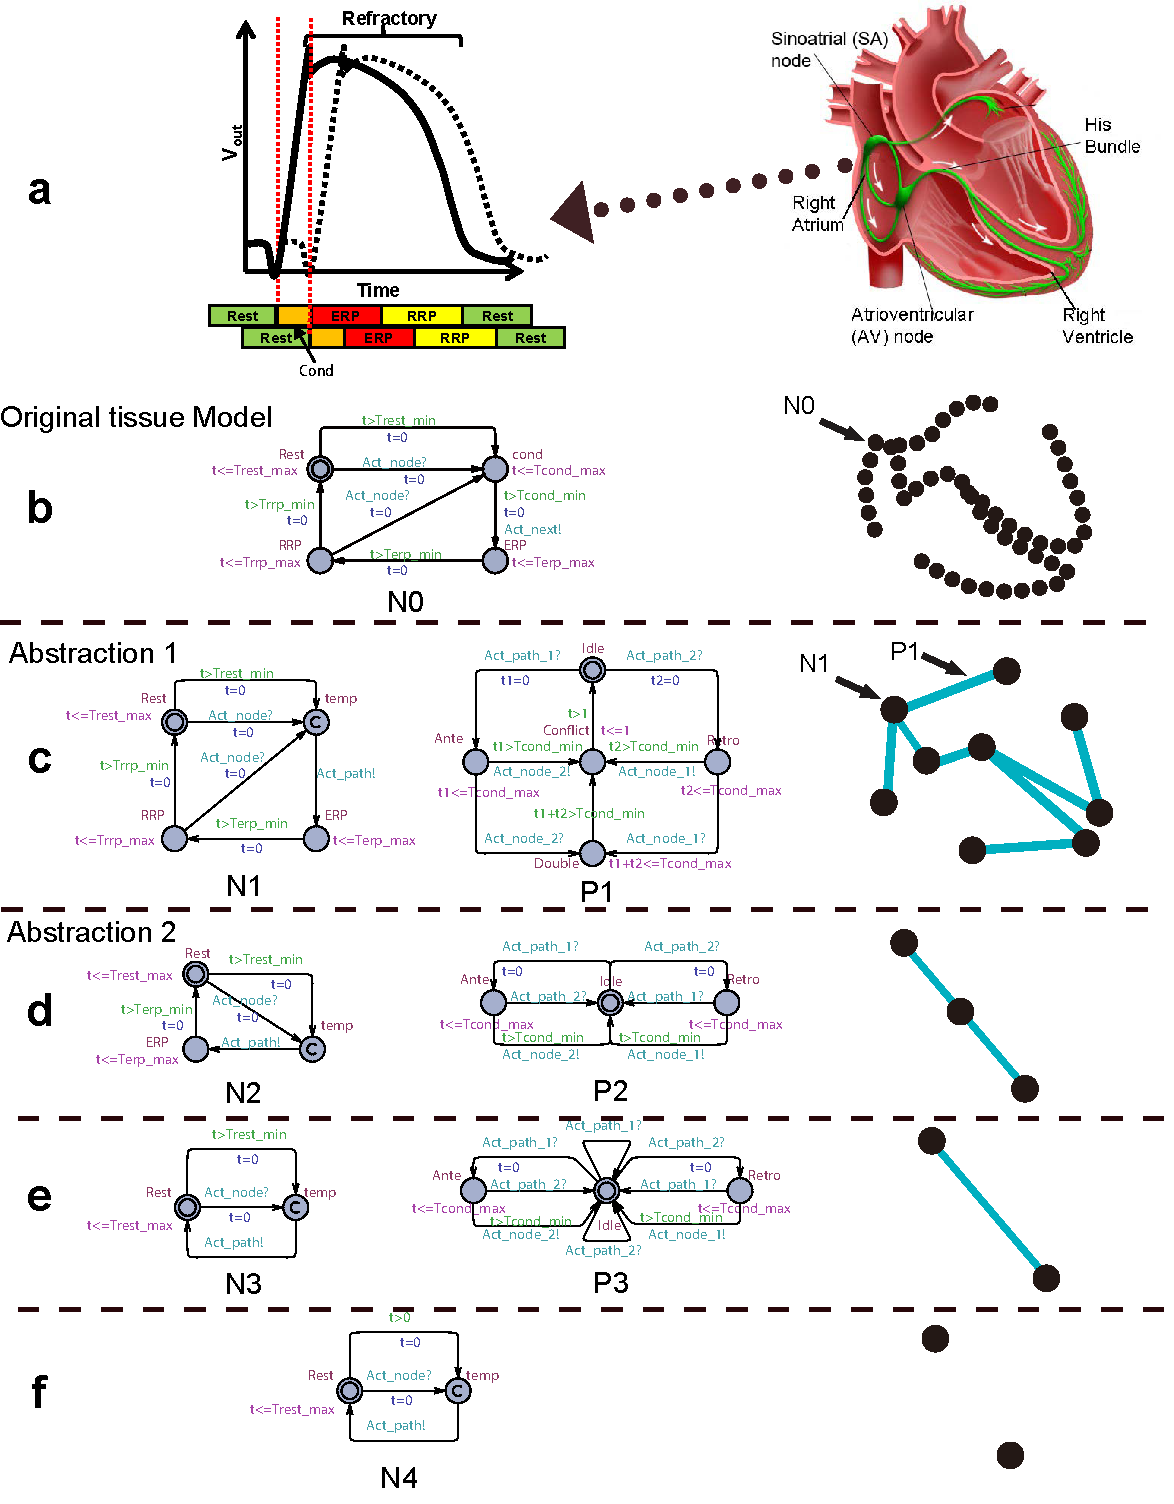
\includegraphics[width=0.9\textwidth]{figs/Heart_abs.pdf}
%\vspace{-10pt}
\caption{(a) Electrical voltage change measured on the heart tissue and its adjacent tissue region (dotted) upon activation. The whole process is divided into timing periods with different behaviors. (b) The original tissue model which captures the refactory timing behaviors of the heart tissue. (c) The conduction property is separated to the path automaton and the heart can be modeled as conduction network. (d) Equivalent locations are merged. (e) The blocking property of the ERP location is replaced by a non-deterministic conduction in the path automaton. (f) Conduction between nodes are replaced by self-activations of the nodes. More details in \cite{STTT13}}
\label{fig:HM_abs}
%\vspace{-10pt}
\end{figure} 
\subsection{Abstraction 1: Abstract Conduction Delays With Paths}
At the first abstraction step, we separate the conduction delay (modeled by the \emph{cond} state in $N0$) from the new node automata $N1$ and model the conduction between two nodes using path automaton $P1$. Since the beat-to-beat dynamics are abstracted with non-determinism, the RRP state is merged with the Rest state in $N1$. The procedure gives us the intuition to abstract the heart as a conduction network as shown in \figref{HM_abs} (c). 

\subsection{Abstraction 2: Merging Equivalent States}
The heart model $H_1'$ still has equivalent locations. In Abstraction 2 we further abstract the node and path automata by merging equivalent states. In the new node automaton $N_2$ we merge the \textsf{RRP} state with the \textsf{Rest} state with:
$$N_2.Trest\_min = N_1.Trest\_min+N_1.Trrp\_min$$
$$N_2.Trest\_max = N_1.Trest\_max+N_1.Trrp\_max$$
Under the assumption that the ERP period of a node automaton is much longer than the conduction delay of a path automaton,  the \textsf{Double} and \textsf{Conflict} location of the path automaton is merged with the \textsf{Idle} state. The heart can be modeled as $H_2=N_2^1\| P_2^1\| N_2^2\| P_2^2\| N_2^3$.

\subsection{Abstraction 3: Replacing Blocking with Non-deterministic Conduction}
In Abstraction 3, we replace the blocking behavior of the \textsf{ERP} location of the node with non-deterministic conduction in the path automaton. There exists a transition\\ 
$RE\| ID\| RE$ 
$\xrightarrow[Act\_path\_1!]{Act\_node\_1?}$ 
$\xrightarrow{Act\_path\_1?}$ 
$RE\| ID\| RE$\\
in $N_3^1\| P_3^1\| N_3^2$ to replace transition\\
$ER\| ID\| ER$ 
$\xrightarrow{Act\_node\_1?}$ 
$ER\| ID\| ER$\\
in $N_2^1\| P_2^1\| N_2^2$

Without the ERP constraint the AV node is no longer needed and the heart can be modeled as $H_3=N_3^1\| P_3\| N_3^2$.  The detailed proof for this timed simulation relation can be found in \cite{STTT13}. 
\subsection{Abstraction 4: Random Heart Model (RHM)}
In Abstraction 4, we further simplify the heart model by removing the conduction path between two nodes. By setting $Trest\_min$ for both nodes to 0 the new heart model $H_4=N_3^1\|N_3^2$ covers all possible behavior of $H_3$. This random heart model with two nodes is the most abstract model that will be used at the beginning of the closed-loop model checking process.
%\textbf{AG}$\varphi\equiv\neg$\textbf{EF}($\neg\varphi$) 

Eventually we have a series of heart models with:

$N_0^1\|N_0^2\cdots N_0^n$\\
$\preceq_t N_1^1\|P_1^1\|N_1^2\cdots P_1^{m}\|N_1^n$\\
$\preceq_t N_1^1\| P_1^1 \| N_1^2\| P_1^2 \| N_1^3$\\
$\preceq_t N_2^1\| P_2^1\| N_2^2\| P_2^2\| N_2^2$\\
$\preceq_t N_3^1\| P_3\| N_3^2$\\
$\preceq_t N_4^1\| N_4^2$

Using this technique, we systematically create a family of heart models with different levels of complexity and expressiveness. In Chapter \ref{ModelChecking} we describe how to balance between complexity and expressiveness and use these heart models for closed-loop model checking of implantable pacemaker.
% \subsubsection{Abstracting Beat-to-beat Dynamics}
% \subsubsection{Abstracting Conduction Delays with Path}
% \subsubsection{Merging Activation-generating Nodes}
% \subsubsection{Replace ERP Blocking With Non-deterministic Conduction}
% \subsubsection{Replace }
\section{Conclusion}
In this chapter, we use heart modeling as example to demonstrate how to develop physiological models for closed-loop evaluation of closed-loop medical devices. We emphasized that models should be developed according to their applications. We developed heart models based on clinical Electrophysiological Testing, and modeled the topological and temporal behaviors of the heart with timed-automata formulation. In the next chapter we will demonstrate the identification and validation of the heart models.




\chapter{Identifying the Environment Model }
\begin{itemize}
	\item What is the importance of model identification?
    \item How to identify?
    \item What's the data availability and quality?
    \item Are there differences for identifying different kind of models?
    \item What are the challenges?
\end{itemize}
Physiological models are developed to represent certain physiological condition in general, or the physiological condition of a specific patient. Therefore the structure of the model and corresponding parameters have to be identified. These information can be obtained from physiological data, which are from: 1) data collected during physiological procedures, and/or 2) physiological literature in which physiological data are analyzed and summarized. Due to limitation on the interactions with the patient, the availability and quality of physiological data are generally bad and there are not enough information to identify all the parameters in the model. It is essential to choose the right level of abstraction so that the model is identifiable (to a large extend). Having physiological correspondence for the model structure and parameters can also simplify the identification process. The rigorousness of the model identification step is also an important factor for the validity of the model. 

In the following sections, we briefly discuss our model identification effort for heart models used in two closed-loop verification applications, and their corresponding challenges. 

\section{Heart Model Identification for Closed-loop Simulation}
In closed-loop simulation, a heart model should be identified to represent a specific patient under certain heart condition. The constraints for model parameters can be obtained from patient data during \emph{ElectroPhysiological (EP) Testing}. During EP testing, the physicians deliver electrical pacing sequence from electrodes placed inside the patient's heart while extracting timing parameters from observed pattern and timing of electrical events. Since the goal for any EP testing procedure is not to determine all the timing parameters for a patient, the amount of parameters that can be identified from the patient data is limited.    

\figref{modelID} illustrates how timing parameters can be extracted during an EP testing procedure. Assume that there are two electrodes placed in the right atrium and right ventricle of the heart respectively (\figref{modelID}.a), and EGM signals can be measured (\figref{modelID}.b). The physician can also apply pacing sequences through the electrodes which can trigger different response from the patient's heart. \figref{modelID}.c shows a heart model structure with unknown parameter values, which can be extracted by analyzing the \emph{timing} and \emph{pattern} of the local activations. 
\begin{figure}[!t]
\centering
		\includegraphics[width=0.9  \textwidth]{figs/modelID.png}
		
%\vspace{-10pt}
\caption{\small (a) Node automaton. Dotted transition is only valid for pacemaker tissue like SA node; (b) Path automaton; (c) Model of the electrical conduction system of the heart using a network of node \& path automata~\cite{vhm_ecrts10}.}
\label{fig:modelID}
%\vspace{-15pt}
\end{figure} 


\section{Heart Model Identification in Closed-loop Model Checking}
In model checking, the heart models in general have simple structure and less parameters due to non-deterministic abstraction. The heart models are developed in consistent with Electrophysiology terminologies, thus each node and path automata and their timing parameters have physiological correspondence which can be found in literature (\cite{josephson}). The range for non-deterministic parameters directly correspond to the range for possible values of corresponding physiological parameters. Therefore model identification for model checking is much simpler. 

An example: \Hao{Need a photo of table of typical parameter values}







\chapter{Validating the Environment Model}
\begin{itemize}
	\item What are the different methods to validate physiological models?
    \item How much confidence can these validation provide?
\end{itemize}
The validity of the environment models affects the validity of the closed-loop verification results. Since models are always approximations of the actual environment, there is always discrepancies between the model and the actual patient (group). The challenge then is to determine how much safety guarantee that model-based closed-loop verification can provide. 

\section{Validate deterministic models}
For deterministic models there are two applications: 1) model a patient with certain heart condition, 2) model a \emph{specific} patient with certain heart condition. For the first application, it is important to show that the model successfully models the underlying mechanism of the heart condition, while for the second application the model should be able to generate same data as the corresponding patient given the same input. 

\subsection{Validating the underlying mechanism}


\begin{figure*}[!t]
\centering
		\subfigure 	[\small Testing result for a real patient (~\cite{josephson})] 
		{
		\includegraphics[width=0.45\textwidth]{figs/WB_book.pdf}
		\label{fig:book_1}
		} 
		\subfigure [\small Testing result for VHM simulation] 
		{	
			\includegraphics[width=0.40\textwidth]{figs/WB_new.pdf} 
			\label{fig:type_1}
		}
\label{fig:Case_1}
%\vspace{-5pt}
\caption{\small Key interval values when the coupling interval shortens for (a) a real patient and (b) in VHM simulation ~\cite{vhm_ecrts10}.}
%\vspace{-15pt}
\end{figure*} 

\subsection{Validating the accuracy of model identification}

% \begin{figure}[\b]
% 	\center
% 	\vspace{-20pt}
% %	\includegraphics[width=0.49\textwidth]{figs/AV_reentry_circuit.pdf}
% 	\includegraphics[width=0.5\textwidth]{figs/AFL_circuit.pdf}
% 	\center
% 	\vspace{-15pt}
% 	\caption{(a) The straight arrow shows the view of the AFL circuit from the right ventricle through the tricuspid valve into the right atrium, while the curved area shows the direction of conduction. (b) The circuit is bounded by the eustachian ridge (ER), connecting the  inferior vena cava (IVC) and the coronary sinus (CS), as well as the crista terminalis (CT), connecting the superior vena cava (SVC) and the IVC. The wavy line shows slow conduction through the CTI, bounded by the ER and the tricuspid valve (\emph{Adapted from} \cite{AFL_diag}). (c) The AFL circuit in the VHM extrapolates nodes and paths from the true physiology. The numbers show the values of conduction timers in the paths, with corresponding slow conduction path on the bottom.}
% 	\label{fig:AFL}
% \end{figure}

\section{Validate by Translating Domain Knowledge**}
For non-deterministic models
\begin{itemize}
	\item The physiological basis for the initial model come from literature
    \item All the abstraction rules follow literature
    \item Models before and after the abstraction have simulation relationships
    \item Ranges of parameters come from literature.
\end{itemize}

 

%\chapter{Physiological Requirements}

Physiological requirements for medical devices specify the closed-loop conditions that the device is designed to achieve with its outputs to the patient. Unlike \emph{specifications} which specify desired device actions in response to the inputs from the patients, physiological requirements focus on the conditions of the patient with and without the device, which would indicate whether the device has fulfilled its intended goals. In this chapter, we address the following questions:
\begin{itemize}
	\vspace{-5pt}
	\item How requirements are different from specifications?
	\vspace{-5pt}
 	\item How can the requirements be represented?
	\vspace{-5pt}
	\item Are all requirements equally important?
\end{itemize}

% \begin{itemize}
% 	\item In contrast to specifications
%     \item Specified on physiological conditions during closed-loop interaction between the patient and the device.
%     \item Timing requirements
%     \item Monitor construction
% \end{itemize}

The most basic requirement for a pacemaker is to maintain the ventricular rate above a minimum level. The corresponding physiological requirement is:
\noindent
 \emph{The interval between two ventricular contractions should always be less or equal to 1000ms.} 

Note that this requirement focuses only on the condition of the patient (ventricular contractions), and there is no mention of the operation of the pacemaker or how the pacemaker should achieve the requirement. Here $1000ms$ is a patient-specific parameter. An example specification of a single chamber pacemaker corresponding to the requirement is:  
\noindent
\emph{If there is no sensed ventricular event 1000ms since the last ventricular event (sensed or paced), the pacemaker should deliver ventricular pacing.}
 
The specification is described using the terminology internal to the pacemaker software (paced and sensed events), and specifies the action of the pacemaker corresponding to certain inputs. For more complex requirements, multiple specifications have to work together to achieve the requirement. Therefore there may exist executions that satisfy all the specifications but not the corresponding requirement. Verifying physiological requirements requires knowledge of the physiological condition and how device interacts with the physiological environment, thus can only be performed in closed-loop. 

Devices are designed to improve certain physiological conditions, the performance of the devices is evaluated on the difference between the patient conditions without the device and with the device. The device should also avoid deteriorating certain patient conditions, thus physiological requirements are specified in the form of:
$$C_{pre}\rightarrow C_{post}$$
in which $C_{pre}$ is the physiological conditions without the device,  and $C_{post}$ is the physiological condition with the device. For model-based closed-loop verification, $C_{pre}$ is often in form of a set of constraints on patient parameters. As a special case, $C_{pre}$ can equal to $true$, means that $C_{post}$ should be satisfied under all possible conditions.

One of the challenges for developing medical device software is to convert physiological requirements, which are generally informal descriptions of physiological conditions, into mathematical descriptions that can be used by verification tools.  In model-based verification, these physiological conditions are mapped onto constraints on model parameters. %In the following section, we use the heart model as example to show this process.

While the device is to aid the physiological function under certain conditions, it must deal with all possible environment conditions. However, in certain extreme conditions, not all physiological requirements can be satisfied due to the limitations of device function. It is thus intuitive to assign priorities to the requirements and assess the capability of the device to prioritize more important requirements in these scenarios. 

We use pacemaker as example to demonstrate how to convert physiological descriptions into mathematical requirements and how priorities of the requirements affect the verification process.

%For convenience, requirements are usually specified with binary results (satisfied/unsatisfied). quantitative
\noindent
\textbf{1. Encoding Physiological Conditions:}  \figref{state} lists example heart conditions and their corresponding constraints on heart model parameters.
\begin{figure}[!t]
	\center
%		\vspace{-10pt}
	\includegraphics[width=0.70\textwidth]{figs/state.pdf}
	\center
	
	\caption{Patient state and equivalence in the heart model}
	\label{fig:state}
\end{figure}
\noindent
\\\textbf{2. Conditional Requirements:} Physiological requirements are in general conditional requirements. Specifying conditional requirements enables tighter constraints on the closed-loop system. \figref{conditional} shows a list of conditional requirements used during the pacemaker case study. 
\begin{figure}
	\center
	\includegraphics[width=0.7\textwidth]{figs/conditional.pdf}
	\center
	\vspace{-10pt}
	\caption{Conditional requirements for the close-loop system}
		%\vspace{-15pt}
	\label{fig:conditional}
\end{figure}
\begin{figure}
	\center
	\includegraphics[width=0.7\textwidth]{figs/properties.pdf}
	\center
	\vspace{-10pt}
	\caption{General requirements for the close-loop system}
		%\vspace{-15pt}
	\label{fig:properties}
\end{figure}
\noindent
\\\textbf{3. Requirement Hierarchy}
For a closed-loop system including a heart $H$ and a pacemaker $P$: $S=H || P$ and two requirements $\varphi_1$ and $\varphi_2$ such that $\mathbb{P}_{\varphi_1}<\mathbb{P}_{\varphi_2}$, the following statement should always hold:
\vspace{-5pt}
$$H\models\varphi_2\rightarrow H||P\models\varphi_2$$
\vspace{-5pt}
meaning if a higher priority requirement is satisfied by the open-loop environment, it should be satisfied by the closed-loop system as well. An example violation of the statement is:
\vspace{-5pt}
$$H\not\models\varphi_1 \&\& H\models\varphi_2 \&\& H||P\models\varphi_1 \&\& H||P\not\models\varphi_2$$
\vspace{-5pt}
which should not be allowed. In our closed-loop verification of pacemaker, the list of physiological requirements with assigned priorities are showing in \figref{properties}.




%\section{Requirement Representations}
%\subsection{TCTL}
%\subsection{Simulink Block}



\chapter{A Dual Chamber Pacemaker Specification}

As part of the model-based design, it is important to have a functional and formal model of the device software for testing and formal verification respectively. In our study, we focus on the implantable  pacemaker since it is one of the simpler implantable cardiac devices as its functionality is based only on timing and does not consider signal morphology. This serves as a good base case to demonstrate the proposed methodology.  In this chapter, we describe the basic specification and formal implementation of a dual chamber pacemaker, as well as a more advanced function on mode switching. The specifications are based on the algorithm descriptions from Boston Scientific manuals (\cite{compass}) and the functional description released as part of the Pacemaker Challenge (\cite{challenge}). 
We aim to answer the following questions here:
\begin{itemize}
	\vspace{-5pt}
	\item How are the pacemaker's timers specified to maintain the appropriate heart rhythm?
	\vspace{-5pt}
   	\item What happens if new functionality is added to the basic model?
\end{itemize}

The artificial pacemaker is designed for patients with bradycardia (i.e. slow heart rate). Two leads, one in the right atrium and one in the right ventricle, are inserted into the heart and fixed onto the inner wall of the heart. These two leads monitors the local activation of the atria and the ventricles, and generate corresponding sensed events \textsf{(AS, VS)} to its software. The software determines the heart condition by measuring time difference between events and delivers pacing events \textsf{(AP, VP)} to the analog circuit when necessary. The analog circuit then delivers pacing signals to the heart to maintain heart rate and A-V synchrony. In order to deal with different heart condition, pacemakers are able to operate in different modes. The modes are labeled using a three character system (e.g. $xyz$). The first position describes the pacing locations, the second location describes the sensing locations, and the third position describes how the pacemaker software responds to sensing. Here we introduce the widely used DDD mode pacemaker which is a dual chamber mode with sensing and pacing in both atrium and ventricle. 

\begin{figure}[!b]
\center
%\vspace{-10pt}
\includegraphics[width=0.85\textwidth]{figs/PM_timers.pdf}
%\vspace{-10pt}
\caption{Basic 5 timing cycles for a dual chamber pacemaker which include the Lower Rate Interval (LRI),  Atrio-Ventricular Interval (AVI), and Upper Rate Interval (URI). Also included are the blanking intervals, Post Ventricular Atrial Refractory Period (PVARP) and Ventricular Refractory Period (VRP), to inhabit action by the pacemaker.}
\label{fig:PMtimers}
%\vspace{-10pt}t

\end{figure} 
\section{Basic Specifications of a DDD Pacemaker}
The DDD pacemaker has five basic timing cycles triggered by external and internal events, as shown in \figref{PMtimers}. We decomposed our pacemaker model into five components which correspond to the five timers. $P=LRI\| AVI\| URI\| PVARP\| VRP$. These components synchronize with each other using broadcast channels and shared variables (as shown in \figref{PMdesign}). 

\subsection{Lower Rate Interval (LRI)}
%\vspace{-5pt}
The Lower Rate Interval (LRI) component is shown in \figref{PMdesign}(a). This component defines the longest interval allowed between two ventricular events, thus keeping the heart rate above a minimum value. In DDD mode, the LRI interval is divided into a V-A interval (TLRI-TAVI) and a A-V interval (TAVI). The LRI component maintains a maximum V-A delay while the AVI component maintains a maximum A-V delay so together they maintain the maximum V-V delay. In the LRI component, the clock is reset when a ventricular event \textsf{(VS, VP)} is received. If no atrial event has been sensed \textsf{(AS)}, the component will deliver atrial pacing \textsf{(AP)} after TLRI-TAVI. 

%\vspace{-5pt}
\subsection{Atrio-Ventricular Interval (AVI) and Upper Rate Interval (URI)}
%\vspace{-5pt}
The function of the AVI component defines the longest interval between an atrial event and a ventricular event. If there is no ventricular event \textsf{(VS)}  within TAVI after an atrial event \textsf{(AS, AP)}, and the time since the last ventricular event \textsf{(VS, VP)} is longer than TURI, the component will deliver ventricular pacing \textsf{(VP)}. The URI limits the ventricular pacing rate by enforcing a lower bound on the times between consecutive ventricle events. The UPPAAL design of AVI and URI component is shown in \figref{PMdesign}(b) and (c).%The UPPAAL design of AVI component is shown in 

%\vspace{-10pt}
\subsection{Post Ventricular Atrial Refractory Period (PVARP) and Post Ventricular Atrial Blanking (PVAB)}
%\vspace{-5pt}
Ventricular events, especially Ventricular Pace \textsf{(VP)} are sometimes so strong that the atrial lead can sense the activation as well. This signal may be falsely recognized as an atrial event and disrupt normal pacemaker function. This scenario is called crosstalk and was discussed in our previous work (\cite{vhm_embc11}). In order to prevent this undesired behavior, and filter potential noises, there is a blanking period (PVAB) followed by a refractory period (PVARP) for the atrial events after each ventricular event \textsf{(VS, VP)}. Atrial events during PVAB are ignored and atrial events during PVARP trigger \textsf{AR!} events which can be used in some advanced diagnostic algorithms. The UPPAAL design of PVARP component is shown in \figref{PMdesign}(d).

%\vspace{-10pt}
\subsection{Ventricular Refractory Period (VRP)}
%\vspace{-5pt}
The VRP follows each ventricular event \textsf{(VP, VS)} to filter noise and early events in the ventricular channel which could otherwise cause undesired pacemaker behavior. \figref{PMdesign}(e) shows the UPPAAL design of VRP component.

\begin{figure}[!t]
\center
%\vspace{-10pt}
\includegraphics[width=0.9\textwidth]{figs/pacemaker.pdf}
%\vspace{-10pt}
\caption{Five basic timing cycles for a dual chamber pacemaker, which include the Lower Rate Interval (LRI), Atrio-Ventricular Interval (AVI), and Upper Rate Interval (URI). Also included are the blanking intervals, Post Ventricular Atrial Refractory Period (PVARP) and Ventricular Refractory Period (VRP), to inhabit action by the pacemaker.}
\label{fig:PMdesign}
%\vspace{-10pt}
\end{figure} 

\section{Mode Switch Operation: Atrial Tachycardia Response}
\label{Mode_switch}
Supraventricular Tachycardia (SVT) is an arrhythmia with an abnormally fast atrial rate. %\figref{SVT} is a series of simulation results for closed-loop interaction between a heart model with SVT and the pacemaker model. The atrial and ventricular channels show electrogram inputs to the pacemaker and the pacemaker channel shows the corresponding events received and generated by the pacemaker software, \cite{vhm_embc11}.
Typically, in a heart without pacemaker, the AV node, which has a long refractory period, can filter most of the fast atrial activations during SVT, thus the ventricular rate remains relatively normal. \figref{SVT_none} demonstrates a pacemaker event trace during SVT, with a pacemaker in ODO mode, which just sensing in both channels. 
As there is no pacing in ODO mode, the heart is in open-loop with the pacemaker. In this particular case, every 3 atrial events (AS) correspond to 1 ventricular event (VS) during SVT. 
As an arrhythmia, SVT is still considered a safe heart condition since the ventricles operate under normal rate and still maintain adequate cardiac output. 

However, in the closed loop case with the DDD pacemaker, the AVI component of a dual chamber pacemaker is equivalent to a virtual pathway in parallel to the intrinsic conduction pathway between the atria and the ventricles. The pacemaker tries to maintain 1:1 A-V conduction and thus increases the ventricular rate inappropriately to match the atrial rate.  This is known as Pacemaker Mediated Tachycardia (PMT) as the heart would have been safe without the pacemaker and its virtual pathway. \figref{SVT_DDD} shows the pacemaker trace of the same SVT case with DDD pacemaker. Although half of the fast atrial events are filtered by the PVARP period ([AR]s), the DDD pacemaker still drives the closed-loop system into 2:1 A-V conduction with faster ventricular rate. Maintaining A-V delay is less important than maintaining an appropriate ventricular rate. The DDD pacemaker violates a higher priority requirement in order to satisfy a lower priority requirement, which is inappropriate.
\begin{figure*}[!t]
\centering
		\subfigure [\small]{			
		\includegraphics[width=0.5  \textwidth]{figs/SVT_none.pdf}
		\label{fig:SVT_none}
		} 
%	\hspace{.1in}%
\vspace{-10pt}
		
		\subfigure [\small] 
		{
		\includegraphics[width=0.5\textwidth]{figs/SVT_DDD.pdf}
		\label{fig:SVT_DDD}
		} 
\vspace{-10pt}
\caption{\small Benign open loop case: SVT without a pacemaker or with a pacemaker in sense-only mode (ODO) (b) Dangerous closed-loop-case SVT with DDD pacemaker which tries to match the fast atrial rate with a corresponding (and dangerous) fast ventricular rate.}
%\vspace{-15pt}
\end{figure*} 

Pacemaker manufacturers have designed algorithms to detect and terminate these behaviors. Intuitively, the mode-switch algorithm first detects SVT. After confirmed detection, it switches the pacemaker from a dual-chamber mode to a single-chamber mode. During the single-chamber mode, the A-V synchrony function of the pacemaker is deactivated thus the ventricular rate is decoupled from the fast atrial rate. After the algorithm determines the end of SVT, it will switch the pacemaker back to the dual chamber mode. 
\begin{figure*}
		\centering
		%\vspace{-19pt}
		\includegraphics[width=0.8\textwidth]{figs/AVI_ms.pdf}
		%\vspace{-10pt}
		\caption{\small (a) After switching to \textsf{VDI} mode, the new LRI component \textsf{LRI'} maintains a minimum V-V interval; (b) After switching to \textsf{VDI} mode, the new AVI component \textsf{AVI'} keeps track of the time after each atrial events.}
		%  \vspace{-20pt}
		\label{fig:avi_ms}
\end{figure*}
The mode-switch algorithm (also known as atrial tachycardia response) specification we use is similar to the one described in the Boston Scientific pacemakers' manual (\cite{compass}). The algorithm first measures the interval between atrial events outside the blanking period (AS, AR). The interval is considered as \emph{fast} if it is above a threshold (\emph{Trigger Rate}) and \emph{slow} otherwise. In our UPPAAL model we model it as $INT$ (see \figref{dur_count} (1)). A counter $CNT$ increments for \emph{fast} events and decrements for \emph{slow} events (see \figref{dur_count} (2)). After the counter value reaches the \emph{Entry Count}, the algorithm will start a \emph{Duration} ($DUR$) ,which is a time interval used to confirm the detection of SVT (see \figref{dur_count} (3)). In the \emph{Duration}, the counter keeps counting. If the counter value is still positive after the \emph{Duration}, the pacemaker will switch to the VDI mode (\emph{Fallback mode}). In the VDI mode, the pacemaker only senses and paces the ventricle. At any time if the counter reaches zero, the \emph{Duration} will terminate and the pacemaker is switched back to DDD mode.
% to show some interesting findings. The basic idea of this simplified model is explained in detail. \\
%\mySubSubSection{UPPAAL model for mode-switch algorithm}
In our UPPAAL model of the mode-switch algorithm, we use nominal parameter values from the clinical setting. We define \emph{trigger rate} at 170bpm (350ms), \emph{entry count} at 8, \emph{duration} for 8 ventricular events and \emph{fallback mode} as VDI. 

In order to model both DDD and VDI modes and the switching between them, we made modifications to the AVI and LRI components.
In each component two copies for both modes are modeled, and switch between each other when switching events (DDD, VDI) are received. During VDI mode, \textsf{VP} is delivered by the LRI component instead of the AVI component. The clock values are shared between both copies in order to preserve essential intervals even after switching. The modified AVI ($AVI'$) and LRI ($LRI'$)components are shown in \figref{avi_ms}. 

\begin{figure*}
		\centering
				%\vspace{-15pt}
		\includegraphics[width=0.9\textwidth]{figs/duration.pdf}
		%\vspace{-10pt}
		\caption{\small (1) Component \textsf{INT}: An atrial event (\textsf{AS,AR}) arrives before \textsf{thresh} after the previous atrial event is regarded as a \textsf{fast} event. Atrial event arrives after \textsf{thresh} and \textsf{AP} are regarded as \textsf{slow} event; (2) Component \textsf{CNT}: After 8 \textsf{fast} event the algorithm will start a duration by sending \textsf{du\_beg} and will switch to \textsf{VDI} mode when the duration ends (\textsf{du\_end}); (3) Component \textsf{DUR} :The duration length is 8 ventricular events (\textsf{VS,VP})}
		  %\vspace{-15pt}
		\label{fig:dur_count}
\end{figure*} 

%%%%%%%%%%%%%%%%%%%%%%%%%%%%%%%%%%%%%%%%%%%%
%%%%%%%%%%%%%%%%%%%%%%%%%%%%%%%%%%%%%%%%%%%%

\chapter{Closed-loop Model Checking}
\label{ModelChecking}
%There are two categories of device bugs: 
%1) the device may fail to conform to its \emph{specifications}, that is, the prescription of how it should react to certain inputs.  
%2) the device may fail to improve the conditions of the patient as promised, even if it conforms to its specifications. 
%The desired physiological conditions that the closed-loop system should achieve are captured in the \emph{physiological requirements}; for example, for a pacemaker, the heart rate should always be maintained above a certain threshold. 
%
%Bugs in the first category (non-conformance to specification) can be detected via systematic and extensive open-loop testing in which a set of input sequences is fed to the device, and its output is compared with the expected output.
%Bugs in the second category (violation of physiological requirements), on the other hand, require the interaction within the \emph{closed-loop system}, which consists of the device and its environment.
%For instance, the pacemaker and the heart as its environment. 
%In the medical device industry, closed-loop verification of the physiological requirements is mostly performed in terms of clinical trials, in which the actual devices are implanted in human subjects over an extended duration.
%Unfortunately, because of the extremely high cost of clinical trials (several million dollars and spanning several years,~\cite{trialcost}), the amount and variety of human subjects during the clinical trials are limited, which reduces the opportunity to find bugs. 
%Moreover, clinical trials are often conducted at the final design stage. Fixing bugs at this stage is very costly.

Model checking is a technique in which the state space of the model under investigation is automatically and exhaustively explored to identify executions or states that violate specified properties. Violations of the properties are returned by the model checkers as \emph{counter-examples}, which can be used by designers to revise the design. In the application of verification of properties in medical devices like implantable pacemaker, model checking can be used to identify known and unknown mechanisms for inducing hazards. This is extended to checking the heart-pacemaker closed-loop models against physiological hazards (e.g. when the pacemaker provides inappropriate therapy which drives the heart to an unsafe state). 

Due to the curse of dimensionality as models get more complex, and hence the large computational cost, there are usually restrictions on the formalism and the complexity of the models under investigation. Using abstract models of the actual system adds the responsibility of proving the conformance between the abstract model and the real system. Assumptions made during abstractions may also introduce false-positives and/or false-negatives into the model checking results. Back in Chapter 2, we introduced a set of heart models with different abstraction levels, that can be used to cover behaviors of physiological conditions using non-determinism. In Chapter 4, we then modeled a dual chamber pacemaker algorithm using timed-automata without doing abstractions. In this chapter, we use model checker UPPAAL to evaluate the pacemaker model against safety properties under different heart conditions captured by the heart models. Techniques to eliminate false-positives by refining the heart models are also discussed. We will try to answer the following questions:
\begin{figure}[!t]
		\centering
		\includegraphics[width=0.8\textwidth]{figs/risk_requirements.pdf}
		\caption{\small Sample Fault Tree Analysis of the physiological conditions leading to the lower rate limit and upper rate limits}
		  %\vspace{-15pt}
		\label{fig:risk_req}
\end{figure}

%            \item What are the effects of adding new features to the software? Can they disrupt the safety properties that the previous device hold?

%In closed-loop model checking, there is only one device model. 
%However there can be a large number of environmental conditions which require different models to represent them. For instance, a heart with atrial flutter has an additional conduction pathway, causing fast atrial rate, that is not present in a healthy heart. The timing and structural differences of different heart conditions should be distinguished in corresponding heart models.
%%\todo[inline]{should we give an example of a heart condition?}
%A set of initial models of the environment can be constructed, but the set is inherently incomplete because of the large number of environment conditions and their combinations. 
%As a result, performing model checking using every model in the set cannot ensure full coverage of the environmental conditions. In the following sections, we will investigate how as we go from basic to more complex requirements, we require more sophisticated approaches to generate and navigate through a variety of environment models. We introduce the concept of an \emph{Abstraction Tree} to systematically encode requirements and choose the appropriate heart models for the requirement. By analyzing the concrete counter-examples we are able to distinguish if the problem is a bug within the device or due to the lack of expressiveness in the environment model. 
\begin{itemize}	
\vspace{-5pt}
	\item How do model checking results fit into the regulation framework?
	\vspace{-5pt}
	\item How do we find the appropriate abstraction level of the environment model for each physiological requirement?
        \vspace{-5pt}
        \item How do we interpret abstract counter-examples returned by model checker?
\end{itemize}
%\section{Testing vs Verification}
%
%\newcommand{\ub}{\bar{u}}
%\newcommand{\yb}{\bar{y}}
%
%\emph{\textbf{Testing}} is a method for checking that a system does indeed obey its specification. 
%In testing, an algorithm will do the following:
%\begin{itemize}
	%\item Initialize the system to some initial state $x_0$ in $X_0$.
	%E.g., for a pacemaker device, this would describe the initial values for the various refractory periods, among other things.
	%\item Generate sequences of input strings $\bar{u}_k$ from some set $A$, in reaction to which the system will produce output strings $\bar{y}_k$,
	%\item A \emph{monitor} logs the output strings and determines whether the pair $(\bar{u}_k,\bar{y}_k)$ satisfies the specification or not.	
%\end{itemize}
%
%Because the set of valid initial states $X_0$ and the set of valid input strings $A$ may be infinite (or simply too large), the test bench must decide on how to intelligently choose a \emph{finite} number of $(x_0,\ub)$.
%They must be chosen such that if the system does not produce wrong behavior with these pairs, then it is unlikely to produce errors under the \emph{full} valid set of pairs, namely, $X_0 \times A$.
%This is the main challenge of testing: how to sample an infinite or large set of behaviors such that it is representative (in the above sense) of the full set of behaviors that $S$ is capable of?
%Another important issue in testing is for how long to test the system: i.e. what should be the length of the $k^{th}$ string $\ub_k$? 
%E.g., if $\ub_k$ has length 1000, the bug might manifest itself on $y_1\ldots y_{1001}$, but not $y_1\ldots y_{1000}$.
%
%Regardless of the testing algorithm, testing remains incomplete, in the sense that short of testing every possible behavior, bugs may lie hidden in the behavior that we did not witness.
%
%\emph{\textbf{Verification}} refers to formal verification.
%It is applicable to finite state systems\footnote{Some infinite-state systems can be formally verified after an abstraction process which essentially produces an equivalent system that has finitely many states.}, 
%and requires formal semantics for the system's operation. 
%Roughly, this means we must have a mathematical unambiguous definition of how the system produces its output.
%A verification algorithm, or \emph{model checker}, will explore the \emph{entire finite state-space} of the system in a systematic manner. 
%Intuitively, if the entire state-space has been explored in all possible ways, and no incorrect behavior has been displayed, then the system is correct. 
%Thus, verification is inherently \emph{complete}: if the model checker determines that the system is correct (under the conditions $A$ and $X_0$), then we can rest assured that is indeed the case.
%Unlike testing, there is no question of whether we missed (didn't run) an initial condition that can display a bug.
%There is also no question of test duration.
%However in practice, some bound on the duration of the verification must be placed to avoid excessively long runs. 
%If the model checker can't determine correctness in that time bound, then the verification is inconclusive.
%
%Verification is computationally expensive and usually more burdensome to setup, but comes with a guarantee on the answer. 
%Testing is computationally cheaper and less burdensome to setup, but the guarantees it provides are significantly weaker.
%Testing, on the other hand, may be the only option for some complex systems that are beyond the capacity of today's model checkers, or which do not possess formal semantics.
%
%In this chapter we cover formal verification of the closed-loop system and address testing in the following chapter.
\section{Risk Analysis for Implantable Pacemaker}
Implantable pacemakers are designed to treat bradycardia by increasing the heart rate with external pacing. Therefore the heart rate should not only be increased to the minimum physiological need, but also should not be increased beyond physiological need. \figref{risk_req} demonstrates two Fault Tree Analysis (FTA) for these two top level hazards. In the remaining chapter we first specify hazards as properties, and use model checking to evaluate whether these hazards have been mitigated by the pacemaker. Then for one of the mitigation algorithm, we examine the mitigation effectiveness and the residue hazard.

\section{Mitigating Top-level Hazards}
The most essential function for the pacemaker is to treat bradycardia by maintaining the ventricular rate above a certain threshold. We define the region where the ventricular rate is slow, as \textsf{unsafe}. The monitor \textsf{PLRI\_test} is designed to measure intervals between ventricular events and is shown in \figref{safety1}. For property
\begin{center}
\textsf{$\varphi_{LRI}=$A[] (PLRI\_test.secV imply PLRI\_test.t$\leq$TLRI)}
\end{center}
we have a closed-loop system  with heart model $H_d$ (described in at the end of Chapter 2): 
$$H_4\| P\| PLRI\_test\models\varphi_{LRI}$$

\begin{figure*}[t]
\centering
%\vspace{-10pt}
		\subfigure[Monitor \textsf{PLRI\_test}] {
				\includegraphics[width=0.5\textwidth]{figs/LRI_test.pdf}
				\label{fig:safety1}
		} 
		\subfigure[Monitor \textsf{PURI\_test}] {	
			\includegraphics[width=0.45\textwidth]{figs/uri_test.pdf}
			\label{fig:uri_test}
		}
		%\vspace{-10pt}
	\caption{(a) Monitor for LRL: Interval between two ventricular events should be less than TLRI, (b) Monitor for URL: Interval between a ventricular event and a VP should be longer than TURI}
\vspace{-10pt}
\end{figure*} 

The pacemaker is not designed to treat tachycardia so it can only pace the heart to increase its rate and cannot slow it down. To mitigate the hazard that the pacemaker may increase the heart rate above physiological need, an Upper Rate Interval (URI) is specified such that the pacemaker can increase the ventricular rate up to this limit. 

\begin{figure}[b]
		\centering
		\includegraphics[width=0.4\textwidth]{figs/vv.pdf}
		\caption{\small Monitor \textsf{Pv\_v} for SVT: There exists an endless sequence in which interval between ventricular events is at most TURI}
		  %\vspace{-15pt}
		\label{fig:vv}
\end{figure}
  
We require that a ventricle pace (VP) can only occur at least $TURI$ after a ventricle event (VS, VP). The monitor \textsf{PURI\_test} is shown in \figref{uri_test}. For the property
\begin{center}
$\varphi_{URI}=$\textsf{A[] (PURI\_test.secV imply PURI\_test.t$\geq$TURI)}
\end{center}
we have: $$H_d\| P\| PURI\_test\models \varphi_{URI}$$

\section{Evaluate the Mitigation}
As described in Chapter \ref{Mode_switch}, the mode switch algorithm has been designed to mitigate the hazard that the A-V synchrony function of DDD pacemaker extends fast
atrial rate to the ventricle. It is important to ensure the effectiveness of the algorithm without inducing other top-level hazards. In this section we first show the existence of the hazard in a pacemaker without the mode-switch algorithm. If the algorithm if effective the hazard will not exist after introducing the algorithm.

\subsection{Existence of Pacemaker Mediated Tachycardia during SVT}
The monitor \textsf{Pv\_v} is designed to show existence of PMT during SVT. It goes to the error state if the ventricular rate drops below the Upper Rate Limit (\figref{vv}).  


We specify 
$\varphi_{MS}=E[] (not Pv\_v.err)$\\
which verifies the existence of PMT. The heart model $H_e$ in Fig. \ref{fig:HM_abs} is not suitable for this property since the non-deterministic conduction of component $P_3$ does not capture the blocking property of the AV node, which is the key in PMT. We use a more refined model $H_d$ which has AV node modeled. To identify the PMT scenario, we first set $H_d.N^1.Trest\_min<100$ so that the atrial rate can be high and $H_d.N^2.Trest\_min>TURI$ so that the intrinsic heart rate is less than TURI. The property is first verified on pacemaker without the mode-switch algorithm. We have $H_d\|P\|Pv\_v\models\varphi_{MS}$ and the evidence returned by the model checker illustrates the PMT scenario.

% There are two separate AVI and LRI components for each mode and switches to the corresponding ones when synchronization signals are received. The clock values are kept so that essential intervals are kept. 
\subsection{Verification against fundamental safety properties}
For a pacemaker with the mode switch algorithm: 

$P_2$=\textsf{LRI'$\|$AVI'$\|$URI$\|$PVARP$\|$VRP$\|$INT$\|$CNT$\|$DUR}, 

we verify the same fundamental safety properties on the pacemaker model with mode-switch algorithm. We have:
$$H_d\|P_2\|PURI\_test\models\varphi_{URI}$$
$$H_d\|P_2\|PLRI\_test\not\models\varphi_{LRI}$$
The Upper Rate Limit property still holds, but the Lower Rate Limit property is violated. The counterexample is proved to be valid after checking the trace of more refined heart models. By analyzing the trace we found that when the pacemaker is switching from VDI mode to DDD mode, the responsibility to deliver VP switched from LRI component to AVI component. Since the clock reference is different (Ventricular events in LRI component and Atrial events in AVI component), the clock value for delivering the next VP is not preserved. As a result, if an atrial event which triggered the mode-switch from VDI to DDD happens within [TLRI-TAVI, TLRI) after the last ventricular event, the next ventricular pacing will be delayed by at most TAVI time, which violates the Lower Rate Limit property (\figref{safety}). 
%%\begin{figure}
%%		\centering
%%		\includegraphics[width=0.4\textwidth]{figs/vv.pdf}
%%		\caption{\small Monitor \textsf{Pv\_v} for SVT: There exists an endless sequence in which interval between ventricular events is at most TURI}
%%		  %\vspace{-15pt}
%%		\label{fig:vv}
%%\end{figure}
\subsection{Verification of the Mode-Switch Algorithm}
After implementing the mode-switch algorithm, we verified the model against the same existence property. We expect the violation of this property, since during VDI mode the ventricular rate of the heart model is less than the Upper Rate Limit and will not trigger ventricular pacing. However, this property is still satisfied, indicating the mode-switch algorithm failed to eliminate the PMT scenario. The evidence trace returned by UPPAAL shows that a subset of atrial events fall into the blanking period after a ventricular event (see \figref{liveness}). As a result, two fast events are reduced to one slow event and mode switch may never happen. This scenario does exist in all our refined heart models, we conclude that the trace is physiologically feasible. The mode-switch algorithm in our pacemaker model can not terminate all PMT behaviors as specified as certain mild PMT events are admissible.
\begin{figure}
\centering
%\vspace{-20pt}
		\subfigure []{
				\includegraphics[width=0.4\textwidth]{figs/safety.pdf}
				\label{fig:safety}
		} 
		\subfigure []{	
			\includegraphics[width=0.4\textwidth]{figs/liveness.pdf}
			\label{fig:liveness}
		}
		\vspace{-10pt}
	\caption{(a) Safety Violation: VP is delayed due to the reset of timer during mode-switch, (b) Correctness Violation: The blocking period may block some atrial events, turning two \emph{Fast} events to one \emph{Slow} event (\cite{TACAS12}})
\vspace{-20pt}
\end{figure} 
\section{Abstraction Tree for Environment Modeling}
In the previous two sections, abstractions and selections of the heart models are performed manually, which require knowledge of both electrophysiology and model checking. 
Counter-examples returned from abstract models can be difficult to interpret by domain experts.
One abstract counter-example could be produced by multiple physiologically valid conditions, which causes ambiguity.
Thus, a rigorous framework is necessary to balance the need to cover a wide range of environmental conditions and the need to provide counter-examples to the physicians within their physiological context. The framework must also allow non-domain experts to perform verification, and establish `hand-off' points where the results of verification can be handed back 
to the experts for interpretation.

In this section, we use a set of domain-specific abstraction rules based on physiological knowledge to ensure the physiological relevance of the behaviors introduced into the abstract models.
The rules are applied to an initial set of physiological models to obtain an abstraction tree, which will be used for closed-loop model checking of the pacemaker. 
A straightforward search procedure is then used to conduct model checking using suitable heart models and return the most concrete and unambiguous counter-examples to the physicians for analysis.
In this framework, physiological knowledge is only needed when constructing the initial model set and when analyzing counter-examples. 
The application of the physiological abstraction rules and the verification procedure can be automated.
The proposed method can potentially be generalized to other domains in which the device operates in a large variety of environmental conditions. More information regarding this research can be found in \cite{regar_tech}.
\subsection*{Step 1: Abstraction Tree construction}
A set of heart models corresponding to different heart conditions are first developed. 
The list can be expanded as new heart conditions are discovered.
Because we start from a set of initial models, and each one may be abstracted using a number of abstraction rules, we have a choice of which rules to apply to which models, and the order in which to apply them. 
Depending on which rule is applied when, we end up with different abstract models.
Thus an \emph{abstraction tree} $T_{HM}$ for the heart is created, as shown in \figref{HM_tree}. 
%Note that applying rules in different order results different abstraction tree. 
%The order used to obtain $HM\_tree$ is based on the domain knowledge that certain heart conditions may have similar behaviors and similar inputs to the pacemaker. 
%This systematic grouping maintains the physiological-relevance of the heart model even at higher abstraction levels, and reduce the necessity to resolve ambiguities at lower abstraction levels when model checking certain requirements.
\begin{figure}[!t]
	\centering
	\includegraphics[width=0.85\textwidth]{figs/abs.pdf}
	%\vspace{-5pt}
	\caption{\small Heart Model Abstraction Tree with arrows showing the direction of the abstraction process starting from detailed models of different heart conditions. Model refinement is in the opposite direction.}
	\vspace{-15pt}
	\label{fig:HM_tree}
\end{figure}

\subsection*{Step 2: Requirement encoding}
The following requirement is designed to prevent the pacemaker from pacing too fast: 
``If the intervals between self-activations of the atria are between 300ms to 1000ms (60bpm - 200bpm), the intervals between ventricular paces should be no shorter than 500ms.''
Self-activation of the atria can be expressed using the location and clock of node automaton $N_A$.
The requirement can be formalized using the monitor  $M_{sing}(VP,500,\infty)$:
%\hatodo{mention $N_A$ is the atrium node automaton}
\[Req1: N_A.loc=Rest \land N_A.t\in [300,1000] \Rightarrow \neg M_{sing}.loc==Err\]
%\todo[inline]{some figure captions are all caps, others are not. please use same thing throughout}
%\begin{figure}[!b]
	%\centering
	%\vspace{-10pt}
	%\includegraphics[width=0.5\textwidth]{figs/abs_sim.pdf}
%
	%\caption{\small Abstraction Rule Application Example}
%\vspace{-10pt}
	%\label{fig:abs_exam}
%\end{figure}
 \subsection*{Step 3: Choosing appropriate heart models for the requirement}
To verify the closed-loop system with pacemaker model $PM$ and abstraction tree $T_{HM}$ (\figref{HM_tree}) against requirement $Req1$, the most abstract appropriate models are selected from the tree. 
The single event monitor $M_{sing}$ from \figref{monitor}(a) with variables $Var(M_{sing})=\{M_{sing}.t,M_{sing}.loc\}$ is used for this requirement. Model checking is performed on the closed-loop system including the heart model $M_H$, the pacemaker model $M_P$, and the monitor $M$. The requirement $\varphi_P$ can be then represented with TCTL formula:
\begin{center}
 \textsf{A[] (not M.Err)}
\end{center}
The variables in the requirement are:
$$Var(Req1)=\{N_A.t,N_A.loc,M_{sing}.loc\}$$
\begin{figure}[b]
		\centering
		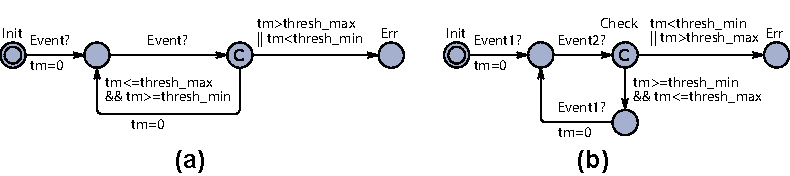
\includegraphics[width=0.8\textwidth]{figs/monitor.pdf}
		%\vspace{-5pt}
		\caption{\small (a) $M_{sing}$ for single event; (b) $M_{doub}$ for two events}
		  \vspace{-10pt}
		\label{fig:monitor}
\end{figure}

At the root of the tree $H_{all}$, we have $\{N_A.t,N_A.loc\} \not \subset Var(H_{all})\cup Var(M_{sing})$. 
So $H_{all}$ is not appropriate for $Req1$. 
All the children of $H_{all}$: $H_n'',H_{at}'''',H_{vt}'''$ are appropriate for $Req1$,
%we have $Var(Req1)\cup Var(M_{sing})\subset Var(H_n'')=Var(H_{at}'''')=Var(H_{vt}''')$, 
thus these three heart models are output as the most abstract models that are appropriate for $Req1$.
\begin{figure}[!t]
	\centering
	\includegraphics[width=0.8\textwidth]{figs/abs_rev.pdf}
	%\vspace{-5pt}
	\caption{\small Model refinement: Finding the most concrete counter-examples using the abstraction tree}
	\vspace{-10pt}
	\label{fig:CE}
\end{figure}
	\vspace{-10pt}
\subsection*{Step 4: Return the most concrete counter-examples}
After the appropriate models for $Req1$ are selected, we have the initial set
$HM=\{H_n'',H_{at}'''',H_{vt}'''\}$.
By model checking on all three initial models in UPPAAL we have: 
$$H_n''||PM\not\models Req1;\; H_{at}''''||PM\not\models Req1;\; H_{vt}'''||PM\not\models Req1$$
%$$[1,[]]=ModelChecking(H_n'',PM,Req1)$$
 %$$[0,CE_1]=ModelChecking(H_{at}'''',PM,Req1)$$
%$$[0,CE_2]=ModelChecking(H_{vt}''',PM,Req1)$$
%\hatodoin{In the following text you use $CE_{at}$, etc. It's  best to use the letter subscripts in the above equations as well, so it's clear which cex comes from which heart model.}
%For the two heart models $H_{at}'''',H_{vt}'''$ in which the requirement is violated, the algorithm keeps going down the abstraction tree, and upon termination counter-examples are returned for the following heart models
The abstraction tree is then further explored. The heart models with counter-examples are illustrated in \figref{CE}, and the most refined heart models with counter-examples are: $H_{n};H_{pvc};H_{af};H_{avn};H_{afib}$.
%$$[0,CE_{at}]=ModelChecking(H_{at},PM,Req1)$$
%$$[0,CE_{pvc}]=ModelChecking(H_{pvc},PM,Req1)$$
%$$[0,CE_{af}]=ModelChecking(H_{af},PM,Req1)$$
%$$[0,CE_{avn}]=ModelChecking(H_{avn},PM,Req1)$$
%$$[0,CE_{afib}]=ModelChecking(H_{afib},PM,Req1)$$

%\begin{figure}[!t]
		%\centering
		%\includegraphics[width=0.9\textwidth]{figs/case.pdf}
		%%\vspace{-5pt}
		%\caption{\small Counter-examples}
		  %\vspace{-10pt}
		%\label{fig:CE}
%\end{figure}
	\vspace{-10pt}
\subsection*{Step 5: Analysis of the counter-examples}
The counter-examples are then shared with physicians for analysis. In \figref{CE} we highlight three counter-examples. In the first counter-example, the intrinsic heart signals over time with up arrows as atrial activations and down arrows as ventricular activations. The signal for the second counter-example shows the pacemaker outputs with up arrows as atrial pacing and down arrows as ventricular pacing.%We only show the activations of the atrial node and ventricle pacing. 

Counter-example $CE_{n}$ is returned by $H_n$ and none of its children models violate the requirement. By careful analysis we found that $CE_{n}$ features the combination of fast intrinsic atrial rate and prolonged A-V conduction delay, which is the combination of heart conditions $H_{st}$ and $H_{av}$. This scenario shows that the abstraction rules can introduce physiological heart conditions that were not explicitly modeled in the initial model set. The pacemaker improved the open-loop heart condition by pacing the ventricles $AVI$ after each atrial event, which is a correct operation of the pacemaker despite the requirement violation. 
%\hatodo{is it TAVI or AVI like in the previous seciton?}

%\hatodoin{Do you mean that $CE_{at}$ is not a bug? Does this mean that the requirement may be violated in ways that are not dangerous?}
Counter-example $CE_{pvc}$ has a very similar execution to $CE_{n}$. However, the activations of the atrial node are triggered by retrograde conduction from ventricle to the atrium initialized by ventricular paces (marker \textsf{cond}). The atrial activations trigger another ventricular pace after $AVI$, which will trigger another retrograde conduction. In this case, the heart rate is inappropriately high, which corresponds to a dangerous closed-loop behavior referred to as \emph{Endless Loop Tachycardia}.

In counter-example $CE_{af}$, the atrial rate is very high, which is also a sub-optimal but not dangerous heart condition. 
However, the ventricular rate can stay normal due to the blocking property of the AV node. 
Despite the filters in the pacemaker, the pacemaker still paces the ventricle for every 3 atrial activations, which extends fast atrial rate to more dangerous fast ventricular rate. 
%\hatodoin{Not very clear..do you mean that the intrinsoc centricular rate is fine because of AV filtering, but the PM is accelarating it?}
This scenario is referred to as Atrial Tachycardia Response of a pacemaker. 

From the analysis, pacemaker operations in $CE_{pvc}$ and $CE_{af}$ must be revised. However, the revision should not affect the behavior in $CE_{n}$. This example demonstrates that counter-examples from refined models provide more physiological context of the requirement violations, and distinguish the physiological conditions that can trigger the violations. The information is helpful for debugging and improving the algorithm. The physicians can also improve the physiological requirement so that these heart conditions can be then considered case by case.\\

\noindent\textbf{Discussion:}\\
Model checking is not widely use in industry, in part, due to scalability issues and also because domain expertise must be a skill possessed by the verification engineer. However, with rigorous abstraction of the system and its environment, model checking can be used to identify 
known and even unknown mechanisms to induce hazards. In this chapter, we use a model of a dual chamber pacemaker as an example to demonstrate the use of model checking during risk analysis. During the process we identified the need to refine the heart models to eliminate false-positives introduced during the abstraction, and demonstrated the difficulty to do so manually. The abstraction tree approach is then proposed to reduce the effort needed for both the developers and the domain experts, which makes model checking a viable approach for providing safety and effectiveness evidence. 




\chapter{Certification}
\begin{itemize}
          	\item What is the current practice for medical device certification? What are the limitations?
          	\item Can model-based closed-loop verification provide more safety guarantee to complement current practice? By how much?
          \end{itemize}
          
\section{Current Practice}
%In United States, medical devices have to be approved by FDA to be released into the market. 
According to their potential risks the devices are categorized into 3 classes, Class I, Class II and Class III, corresponding to low-risk, medium-risk and high-risk devices \cite{class}. Life-sustaining devices like implantable pacemakers are classified as Class III and in general are subject to the most strict regulations.

There are two processes that a medical device can enter the market in U.S.: the Premarket Notification, also known as 510(k) \cite{510k}, and the Pre-Market Approval (PMA) \cite{PMA}. In a 510(k) submission the device manufacturers are only required to provide evidence that the device is \emph{substantial equivalent} to a \emph{predicate device}, which has been approved for the market. Therefore, the 510(k) submission does not directly require clinical evidence for the safety and effectiveness of the device, thus is suitable for mostly low-risk devices like Class I and Class II devices.  The Pre-Market Approval (PMA) submission is a more stringent regulatory process in which direct clinical evidence is required to prove the safety and effectiveness of the device. However, not all Class III devices are subject to PMA submission. If a Class III device clears the 510(k) process and FDA has not requested PMA for that device, the device is still cleared for market release. A study shows that for Class III devices which PMA has been requested, the levels of evidence varies. Only 40\% of the PMA submissions are supported by controlled clinical trials, which provide the most rigorous clinical evidence \cite{cert_prob}. The lack of quality evidence is usually due to the high cost of the controlled clinical trials.
\section{Evidence from Model-based Design}
%\cite{pancreas}
Model-based verification provides a low-cost solution to provide reasonable evidence for the safety and effectiveness of the devices. The open questions are:

\begin{itemize}
	\item How valid are the models?
	\item How much confidence can they provide?
\end{itemize}



\backmatter




\renewcommand{\bibname}{References}

\bibliographystyle{plainnat}
\bibliography{bibliography}

\end{document}